\ifdefined\included
\else
\documentclass[a4paper,11pt,twoside]{StyleThese}
\usepackage{amsmath,amssymb, amsthm}             % AMS Math
\usepackage[T1]{fontenc}
\usepackage[utf8x]{inputenc}
\usepackage{babel}
\usepackage{datetime}

\usepackage{silence}

\WarningFilter{minitoc(hints)}{W0023}
\WarningFilter{minitoc(hints)}{W0028}
\WarningFilter{minitoc(hints)}{W0030}

\usepackage{lmodern}
\usepackage{tabularx}
%\usepackage{tabular}
\usepackage{multirow}
\usepackage{xspace}

\usepackage{subfig}
\usepackage[inline]{enumitem}

\usepackage{hhline}
\usepackage[left=1.5in,right=1.3in,top=1.1in,bottom=1.1in,includefoot,includehead,headheight=13.6pt]{geometry}
\renewcommand{\baselinestretch}{1.05}

% Table of contents for each chapter

\usepackage[nottoc, notlof, notlot]{tocbibind}
\usepackage{minitoc}
\setcounter{minitocdepth}{2}
\mtcindent=15pt
% Use \minitoc where to put a table of contents

\usepackage{aecompl}

% Glossary / list of abbreviations

\usepackage[intoc]{nomencl}
\iftoggle{ThesisInEnglish}{%
\renewcommand{\nomname}{Glossary}
}{ %
\renewcommand{\nomname}{Liste des Abréviations}
}

\usepackage{etoolbox}
\renewcommand\nomgroup[1]{%
  \item[\bfseries
  \ifstrequal{#1}{A}{Number Sets}{%
  \ifstrequal{#1}{G}{Agents Beliefs and Action Models}{%
  \ifstrequal{#1}{N}{Navigation}{%
  \ifstrequal{#1}{O}{Ontology}{%
  \ifstrequal{#1}{R}{Referring Expression Generation}{%
  \ifstrequal{#1}{Z}{Controllable and Uncontrollable Agents Task Planning}{}}}}}}%
]}

\makenomenclature



% My pdf code

\usepackage{ifpdf}

\ifpdf
  \usepackage[pdftex]{graphicx}
  \DeclareGraphicsExtensions{.jpg}
  \usepackage[pagebackref,hyperindex=true]{hyperref}
  \usepackage{tikz}
  \usetikzlibrary{arrows,shapes,calc}
\else
  \usepackage{graphicx}
  \DeclareGraphicsExtensions{.ps,.eps}
  \usepackage[dvipdfm,pagebackref,hyperindex=true]{hyperref}
\fi

\graphicspath{{.}{images/}}

%% nicer backref links. NOTE: The flag ThesisInEnglish is used to define the
% language in the back references. Read more about it in These.tex

\iftoggle{ThesisInEnglish}{%
\renewcommand*{\backref}[1]{}
\renewcommand*{\backrefalt}[4]{%
\ifcase #1 %
(Not cited.)%
\or
(Cited in page~#2.)%
\else
(Cited in pages~#2.)%
\fi}
\renewcommand*{\backrefsep}{, }
\renewcommand*{\backreftwosep}{ and~}
\renewcommand*{\backreflastsep}{ and~}
}{%
\renewcommand*{\backref}[1]{}
\renewcommand*{\backrefalt}[4]{%
\ifcase #1 %
(Non cité.)%
\or
(Cité en page~#2.)%
\else
(Cité en pages~#2.)%
\fi}
\renewcommand*{\backrefsep}{, }
\renewcommand*{\backreftwosep}{ et~}
\renewcommand*{\backreflastsep}{ et~}
}

% Links in pdf
\usepackage{color}
\definecolor{linkcol}{rgb}{0,0,0.4} 
\definecolor{citecol}{rgb}{0.5,0,0} 
\definecolor{linkcol}{rgb}{0,0,0} 
\definecolor{citecol}{rgb}{0,0,0}
% Change this to change the informations included in the pdf file

\hypersetup
{
bookmarksopen=true,
pdftitle="Endowing the robot with the abilities to control and evaluate its contribution to a human-robot joint action",
pdfauthor="Amandine MAYIMA", %auteur du document
pdfsubject="Thèse", %sujet du document
%pdftoolbar=false, %barre d'outils non visible
pdfmenubar=true, %barre de menu visible
pdfhighlight=/O, %effet d'un clic sur un lien hypertexte
colorlinks=true, %couleurs sur les liens hypertextes
pdfpagemode=None, %aucun mode de page
pdfpagelayout=SinglePage, %ouverture en simple page
pdffitwindow=true, %pages ouvertes entierement dans toute la fenetre
linkcolor=linkcol, %couleur des liens hypertextes internes
citecolor=citecol, %couleur des liens pour les citations
urlcolor=linkcol %couleur des liens pour les url
}

% definitions.
% -------------------

\setcounter{secnumdepth}{3}
\setcounter{tocdepth}{2}

% Some useful commands and shortcut for maths:  partial derivative and stuff

\newcommand{\pd}[2]{\frac{\partial #1}{\partial #2}}
\def\abs{\operatorname{abs}}
\def\argmax{\operatornamewithlimits{arg\,max}}
\def\argmin{\operatornamewithlimits{arg\,min}}
\def\diag{\operatorname{Diag}}
\newcommand{\eqRef}[1]{(\ref{#1})}

\usepackage{rotating}                    % Sideways of figures & tables
%\usepackage{bibunits}
%\usepackage[sectionbib]{chapterbib}          % Cross-reference package (Natural BiB)
%\usepackage{natbib}                  % Put References at the end of each chapter
                                         % Do not put 'sectionbib' option here.
                                         % Sectionbib option in 'natbib' will do.
\usepackage{fancyhdr}                    % Fancy Header and Footer

% \usepackage{txfonts}                     % Public Times New Roman text & math font
  
%%% Fancy Header %%%%%%%%%%%%%%%%%%%%%%%%%%%%%%%%%%%%%%%%%%%%%%%%%%%%%%%%%%%%%%%%%%
% Fancy Header Style Options

\pagestyle{fancy}                       % Sets fancy header and footer
\fancyfoot{}                            % Delete current footer settings

%\renewcommand{\chaptermark}[1]{         % Lower Case Chapter marker style
%  \markboth{\chaptername\ \thechapter.\ #1}}{}} %

%\renewcommand{\sectionmark}[1]{         % Lower case Section marker style
%  \markright{\thesection.\ #1}}         %

\fancyhead[LE,RO]{\bfseries\thepage}    % Page number (boldface) in left on even
% pages and right on odd pages
\fancyhead[RE]{\bfseries\nouppercase{\leftmark}}      % Chapter in the right on even pages
\fancyhead[LO]{\bfseries\nouppercase{\rightmark}}     % Section in the left on odd pages

\let\headruleORIG\headrule
\renewcommand{\headrule}{\color{black} \headruleORIG}
\renewcommand{\headrulewidth}{1.0pt}
\usepackage{colortbl}
\arrayrulecolor{black}

\fancypagestyle{plain}{
  \fancyhead{}
  \fancyfoot{}
  \renewcommand{\headrulewidth}{0pt}
}

%\usepackage{MyAlgorithm}
%\usepackage[noend]{MyAlgorithmic}
\usepackage{algorithm}
\usepackage[noend]{algpseudocode}
\usepackage{comment}
\usepackage[ED=MITT-InfoTel, Ets=INSA]{tlsflyleaf}
%%% Clear Header %%%%%%%%%%%%%%%%%%%%%%%%%%%%%%%%%%%%%%%%%%%%%%%%%%%%%%%%%%%%%%%%%%
% Clear Header Style on the Last Empty Odd pages
\makeatletter

\def\cleardoublepage{\clearpage\if@twoside \ifodd\c@page\else%
  \hbox{}%
  \thispagestyle{empty}%              % Empty header styles
  \newpage%
  \if@twocolumn\hbox{}\newpage\fi\fi\fi}

\newcommand*{\algrule}[1][\algorithmicindent]{%
	\makebox[#1][l]{%
		\hspace*{.2em}% <------------- This is where the rule starts from
		\vrule height .75\baselineskip depth .25\baselineskip
	}
}

%%% to have lines in algorithm, from stackexchange
\newcount\ALG@printindent@tempcnta
\def\ALG@printindent{%
	\ifnum \theALG@nested>0% is there anything to print
	\ifx\ALG@text\ALG@x@notext% is this an end group without any text?
	% do nothing
	\else
	\unskip
	% draw a rule for each indent level
	\ALG@printindent@tempcnta=1
	\loop
	\algrule[\csname ALG@ind@\the\ALG@printindent@tempcnta\endcsname]%
	\advance \ALG@printindent@tempcnta 1
	\ifnum \ALG@printindent@tempcnta<\numexpr\theALG@nested+1\relax
	\repeat
	\fi
	\fi
}
% the following line injects our new indent handling code in place of the default spacing
\patchcmd{\ALG@doentity}{\noindent\hskip\ALG@tlm}{\ALG@printindent}{}{\errmessage{failed to patch}}
\patchcmd{\ALG@doentity}{\item[]\nointerlineskip}{}{}{} % no spurious vertical space
% end vertical rule patch for algorithmicx

\makeatother
 
%%%%%%%%%%%%%%%%%%%%%%%%%%%%%%%%%%%%%%%%%%%%%%%%%%%%%%%%%%%%%%%%%%%%%%%%%%%%%%% 
% Prints your review date and 'Draft Version' (From Josullvn, CS, CMU)
\newcommand{\reviewtimetoday}[2]{\special{!userdict begin
    /bop-hook{gsave 20 710 translate 45 rotate 0.8 setgray
      /Times-Roman findfont 12 scalefont setfont 0 0   moveto (#1) show
      0 -12 moveto (#2) show grestore}def end}}
% You can turn on or off this option.
% \reviewtimetoday{\today}{Draft Version}
%%%%%%%%%%%%%%%%%%%%%%%%%%%%%%%%%%%%%%%%%%%%%%%%%%%%%%%%%%%%%%%%%%%%%%%%%%%%%%% 

\newenvironment{maxime}[1]
{
\vspace*{0cm}
\hfill
\begin{minipage}{0.5\textwidth}%
%\rule[0.5ex]{\textwidth}{0.1mm}\\%
\hrulefill $\:$ {\bf #1}\\
%\vspace*{-0.25cm}
\it 
}%
{%

\hrulefill
\vspace*{0.5cm}%
\end{minipage}
}

\let\minitocORIG\minitoc
\renewcommand{\minitoc}{\minitocORIG \vspace{1.5em}}

\usepackage{multirow}
%\usepackage{slashbox}

\newenvironment{bulletList}%
{ \begin{list}%
	{\tiny$\bullet$}%
	{\setlength{\labelwidth}{25pt}%
	 \setlength{\leftmargin}{30pt}%
	 \setlength{\itemsep}{-0.5em}}}%
{ \end{list} }

\newenvironment{inlineEnumerate}
{\begin{enumerate*} [label={(\arabic*)}] }
{\end{enumerate*}}

\theoremstyle{definition}
\newtheorem{definition}{Definition}
\renewcommand{\epsilon}{\varepsilon}

% centered page environment

\newenvironment{vcenterpage}
{\newpage\vspace*{\fill}\thispagestyle{empty}\renewcommand{\headrulewidth}{0pt}}
{\vspace*{\fill}}

\newenvironment{asl}{\ttfamily\begin{tabbing}~~~\=$\leftarrow$ \= ~~~ \=
		\kill}{\end{tabbing}}

\usepackage{tablefootnote}

\theoremstyle{plain}
\newtheorem{constraint}{Constraint}[section]

\algnewcommand\algorithmicforeach{\textbf{for each}}
\algnewcommand\algorithmicin{\textbf{in}}
\algdef{S}[FOR]{ForEach}[2]{\algorithmicforeach\ #1\ \algorithmicin\ #2\ \algorithmicdo}

\algnewcommand\algorithmicforkxor{\textbf{do fork-join-xor}}
\algnewcommand\algorithmicendforkxor{\textbf{end fork-join-xor}}
\algdef{SE}{ForkXor}{EndForkXor}{\algorithmicforkxor}{\algorithmicendforkxor}


\usepackage{listings}
\lstset{
	frame=single,
	captionpos=b,
	breaklines=true,
	basicstyle=\ttfamily,
	numberstyle=\color{black},
	tabsize=2,
	mathescape=true,
	literate=%
		{â}{{\^a}}1
}

\lstdefinestyle{inline}{
	frame=none,
	aboveskip=\smallskipamount,
	belowskip=\smallskipamount,
}

\lstdefinestyle{OwlTurtle}{
	language=C,
	tabsize=4,
	basicstyle=\scriptsize\ttfamily,
	keywordstyle=\bfseries\color{darkgray},
	morekeywords={rdf:type, rdfs:domain, rdfs:subPropertyOf, rdfs:range, :hasSubtask, :DecompositionUsedBy, rdfs:subClassOf, :hasDecomposition, owl:inverseOf, htn_actions:hasEffect, rdfs:label},
	alsoletter=:
}

\lstdefinestyle{aslDef}{
	frame=none,
%	breaklines=false,
	%xleftmargin=.1\textwidth, xrightmargin=.1\textwidth
}

\fancypagestyle{example}{%
	\fancyhead[LE]{\bfseries\thepage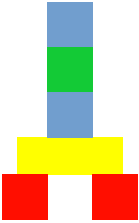
\includegraphics[scale=0.20]{figures/chapter2/task_goal.pdf}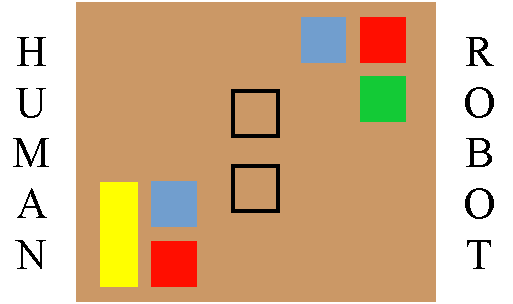
\includegraphics[scale=0.18]{figures/chapter2/task_setup_mini.pdf}}   
	\fancyhead[RO]{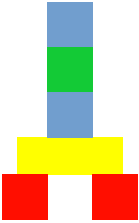
\includegraphics[scale=0.20]{figures/chapter2/task_goal.pdf}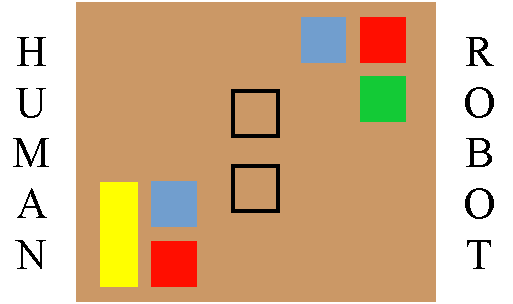
\includegraphics[scale=0.18]{figures/chapter2/task_setup_mini.pdf}\bfseries\thepage}  
	\fancyhead[RE]{\bfseries\nouppercase{\leftmark}}      % Chapter in the right on even pages
	\fancyhead[LO]{\bfseries\nouppercase{\rightmark}}     % Section in the left on odd pages
}%

\usepackage{pdfpages}
\usepackage{makecell}
\usepackage{pdflscape} 
\usepackage{mathtools}
\usepackage[section]{placeins}
\usepackage{afterpage}

%%%%%%%% my commands
\newcommand{\etal}{\textit{et al}.}
\newcommand{\ie}{\textit{i.e.}, }
\newcommand{\eg}{\textit{e.g.}, }
\newcommand{\fact}[3]{\mbox{\textit{#1}(#2, #3)}}
\newcommand{\circledtext}[1]{\raisebox{.5pt}{\textcircled{\raisebox{-.9pt} {#1}}}}
\newcommand{\sparql}{\textsc{SPARQL}}

\newcommand{\algConst}[1]{${\scriptscriptstyle #1}$}
\newcommand{\algNormTextSub}[2]{$\text{#1}_{#2}$}

\newcommand{\aslnumber}[1]{$#1$}
\newcommand{\aslstring}[1]{\textsf{#1}}
\newcommand{\aslvar}[1]{\textcolor{purple}{\textit{#1}}}
\newcommand{\asllabel}[1]{\textbf{#1}}
\newcommand{\annotation}[1]{{\footnotesize #1}}
\newcommand{\rulebody}[1]{\mbox{\hspace{.05\linewidth}}\begin{minipage}[t]{0.9\linewidth}#1.\end{minipage}}
\newcommand{\context}[1]{\begin{minipage}[t]{0.9\linewidth}#1\end{minipage}}
\newcommand{\planbody}[1]{\begin{minipage}[t]{0.9\linewidth}#1.\end{minipage}}
\newcommand{\Jason}[0]{\textbf{\textit{Jason}}}
\newcommand{\sn}{\mbox{\large\textbf{\texttt{\textasciitilde}}}}


\sloppy
\begin{document}
\setcounter{chapter}{1} %% Numéro du chapitre précédent ;)
\dominitoc
\faketableofcontents
\fi

\chapter{Joint Action-based Human-Aware supeRVISor: JAHRVIS}
\label{chapter:chap2}
\chaptermark{JAHRVIS}
\minitoc

\section{The Role and Features of JAHRVIS}\label{chap2:sec:sup_features}

We defined two roles for \acrfull{jahrvis}, the Supervision component: to be able to control the robot's actions and behavior in a human-robot joint action, and to be able to evaluate if this interaction is going well or not. This latter should enhance the decision-making, giving an additional data to take into account. 

\acrshort{jahrvis} is a supervision system, \ie it embeds the robot high-level decisions, controls its behavior and tries to react to contingencies, always considering the human it is interacting with. It is able to do so by taking into account shared plans, human mental states, its knowledge about the current state of the environment, and human actions. The module to monitor and recognize these actions is model-based and allows to take into account a potentially unreliable perception of the human. JAHRVIS is designed in such a way that it is generic enough to handle various kinds of tasks. It can also manage  different kinds of human-robot shared plans as input: shared plans for which actions might not be allocated to an agent at planning time and objects might be referred to with a semantic query, and conditional shared plans which anticipate different possibilities for the human decision/action. This modality dedicated to decision-making and control will be presented in Section~\ref{chap2:sec:control}.

Not only \acrshort{jahrvis} controls the robot contribution to a collaborative task, it also tries to evaluate if the interaction is going well or not. It is possible thanks to a set of metrics we have built and a method to aggregate them. We claim that having a robot with this ability allows it to enhance and make more pertinent its decision-making processes. The evaluation of the Quality of Interaction (QoI) relies on a model of interaction, considered at  three levels: the interaction session level, the tasks level and the actions level. In future work, this granularity will allow the robot to know precisely on what level it needs to act when a low QoI is assessed. Indeed, for instance, a task can be of poor quality while the session can still be considered as going well. QoI principles and metrics will be described in Section~\ref{chap2:sec:qoi}.

A part of the control features presented here is inspired from Sandra Devin~\cite{devin_2017_decisional}. Indeed, we intended to pursue her work, re-implementing a part of her software using a more friendly framework, \ie with Jason instead of if/else statements in C++, giving our software more flexibility, readability and genericness.
Then, to go further, we developed \acrshort{jahrvis}, a more complete approach of a supervision component dedicated to HRI which tries to satisfy multiple objectives:

\begin{bulletList}
	\item \textbf{Be generic}. The objectives developed in the rest of list are to reach for most collaborative tasks. Thus, it seemed essential to us to develop a software not dedicated to a particular human-robot task but able to handle plans for varied tasks. 
	\item \textbf{Consider the human partner}. In HRI, the human and the robot are partners. As seen in Section~\ref{chap1:sec:ja}, partners perform better when taking the other into account. Thus, by considering human abilities, perspective and mental states, the supervisor makes the robot a better partner for the human.
	\item \textbf{Leave some decisions to the human}. In some cases, it is not useful, nay counterproductive that the robot plans all the human action parameters beforehand, who should execute a given action when it does not matter, or the order in which some actions should be executed. Thus, we propose a supervisor handling two types of plan allowing to latitude to human decisions and actions: conditional plans, and plans extending ``Agent X'' shared plans~\cite{devin_2017_decisions}.
	\item \textbf{Monitor human actions}. To monitor the plan progress, the robot should be able to monitor the human, \ie recognize their actions or be able to tell if they are idle.
	\item \textbf{Handle contingencies}. The robot has a shared plan but it is not sure that the human has exactly the same, or failures can happen (see Section~\ref{chap1:sec:failures}). Therefore, sometimes not everything is like the robot had planned. Thus, it should be able to handle a certain amount of contingencies.
	\item \textbf{Do relevant communications}. As stated in Section~\ref{chap1:subsec:comm}, communication is one of the key of collaboration. Therefore, it is important to endow the robot with the ability to perform relevant communication actions, verbal and non-verbal.
	\item \textbf{Considerate the interaction session level} A robot dedicated to collaborative tasks, in a real-life context, will interact with humans outside or between these tasks. We propose to consider this fact by defining what we called \textit{interaction sessions}. An interaction session gives a frame to the interaction and allow to take into account a number of facts from one task to another or from one session to another.
	\item \textbf{Evaluate the quality of the interaction}. Enriching the robot knowledge with a good estimation about how the interaction is going, can enhance its decision-making process and thus, its social behaviour.
	\item \textbf{Adapt to the human experience, abilities or preferences}. Humans are all different, because of their experience, abilities or preferences among other things. A robot taking into account its previous interactions with a human (\eg behaving differently with a novel user or an experienced user) or adapting to their abilities (\eg some people cannot climb stairs, a robot guide can indicate the elevator instead) will improve the efficiency and the quality of the interaction, and the user's experience.
\end{bulletList}


\section{An Overview of our Robotic Architecture}\label{chap2:sec:rob_archi}

In this section, we will shortly present an overview of the robotic architecture that has been developed inside the RIS team of LAAS-CNRS. The purpose of this overview is to give the reader inform the reader about the inputs available for the supervision software, \acrshort{jahrvis}. Two instantiations of this architecture for two different tasks will be described in Chapter~\ref{chapter:chap3} and Chapter~\ref{chapter:chap4}. This architecture model, shown in Figure~\ref{chap2:fig:archi}, is a descendant of the architecture developed by Lemaignan and colleagues~\cite{lemaignan_2017_artificial}, mentioned in Section~\ref{chap1:subsec:archi}. 

\begin{figure}[!ht]
	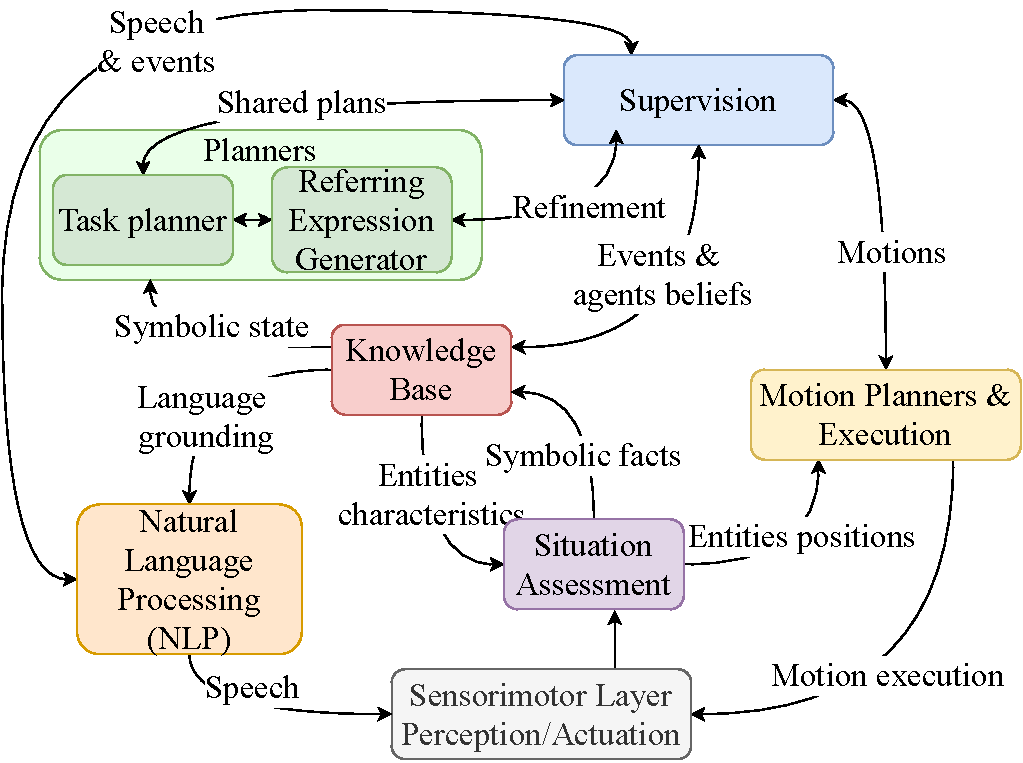
\includegraphics[width=\linewidth]{figures/chapter2/archi_overview.pdf}
	\caption{Overview of the RIS architecture}
	\label{chap2:fig:archi}
\end{figure}


\subsection{Situation Assessment}
The Situation Assessment has two roles:
\begin{enumerate}
	\item  to gather different perceptual information and build an internal geometric representation of the world, composed of objects and agents; from this world representation, the module runs reasoning processes to interpret it in terms of symbolic statements between the objects themselves and between the involved agents and the objects,
	\item estimate the human's perspective and build an estimation of their world representation; it is the first step allowing to implement the theory of mind principles \cite{baron_1985_does}
\end{enumerate}

Thus, the Situation Assessment outputs data, which we call \textit{symbolic facts}, such as \fact{isOnTopOf}{cube\_1}{cube\_3} or \fact{isReachableBy}{cube\_2}{human\_0}.

\subsection{Knowledge Base}

During an interaction, each agent has their knowledge base, as they can have belief divergences. A Knowledge Base is divided into two parts :
\begin{enumerate}
	\item The \textit{semantic} part is in charge of representing the environment elements meaning, the objects' and agents' types, their applicable properties, the descriptions and parameters of the actions, a part of the language model with verbs or pronouns, and their names in natural language. Besides, it is also in charge of representing the current symbolic world-state (the computed facts) and thus the instantiation of the concepts in terms of physical (\eg this particular block) or abstract (\eg this particular action instance) entities.
	\item  The \textit{episodic} part is a timeline, keeping track of the symbolic facts computed over time.
\end{enumerate}

The Supervisor can subscribe to a given type of fact, allowing to receive every fact update of this type (\eg the Supervisor can ask to receive every update (addition or deletion) of any fact belonging to the type \fact{isOnTopOf}{Cube}{Table}). It can also query a information when needed (\eg the Supervisor can ask the human understandable name of pick\_action which is pick).

\subsection{Motion Planner}
The Motion Planner allows the robot to execute actions, such as pick and place, and also to navigate in its environment. To do so, it generates a plan for the move when requested by the Supervisor and then execute it. It sends feedbacks about the current execution, \eg when something goes wrong or estimated remaining time of execution.

\subsection{Task Planner}
The Task Planner can generate a shared plan in which each agent, human and robot, has actions of the task assigned to them, depending on some criteria. However, the human is neither an agent that the planner can directly control or an agent that will know the complete plan. Thus, it allows the robot to plan by emulating the human decision, action, and reaction processes. 

\subsection{Supervision}
The Supervision is the puppet master of the system, embedding the robot high-level decisions, controls its behavior and tries to react to contingencies, always considering the human it is interacting with. It is not standalone, relying on the components described above to be able to take decisions, be aware of the environment and make the robot moves.
\newline

After giving an overview of the components on which the supervision relies, we present the context in which we place ourselves for human-robot collaboration.

\section{Representation of a H-R collaborative activity}\label{chap2:sec:levels}\todo{modifs à faire}
It is possible to describe and decompose a Human-Robot collaborative activity in various ways. For all the following definitions, we place ourselves in the context of one-to-one human-robot interactions, however we  believe that the scheme can be extended to multi-human multi-robot contexts. 
We draw our inspiration from the literature of sociology and robotics to define a model of interaction with three layered levels: interaction session, tasks and actions; as illustrated in Fig.~\ref{fig:levels}. We chose to represent collaborative tasks and their decomposition using the \acrfull{htn}~\cite{ghallab_2016_automated} representation which is often used in cognitive robotics~\cite{ingrand-2017,lallement_2014_hatp, buisan_2021_human} and because it allows to deal with goal-based and situation-based activities at different levels of hierarchy such as task, subtasks and actions and consequently to consider different level of granularity. In the example of a task with an overall bad Quality of Interaction, it would be interesting to know that in fact it is only a particular action or subtask ruining it. Indeed, the other parts of the task can be ok, or on the opposite, a particular subtask or action can have performed very well among the others. We need and use this granularity also on three levels defined (interaction session, tasks and actions) to finely evaluate the Quality of Interaction, as a task can be of poor quality but the session is globally going well. 

\begin{figure}[!ht]
	\centering
	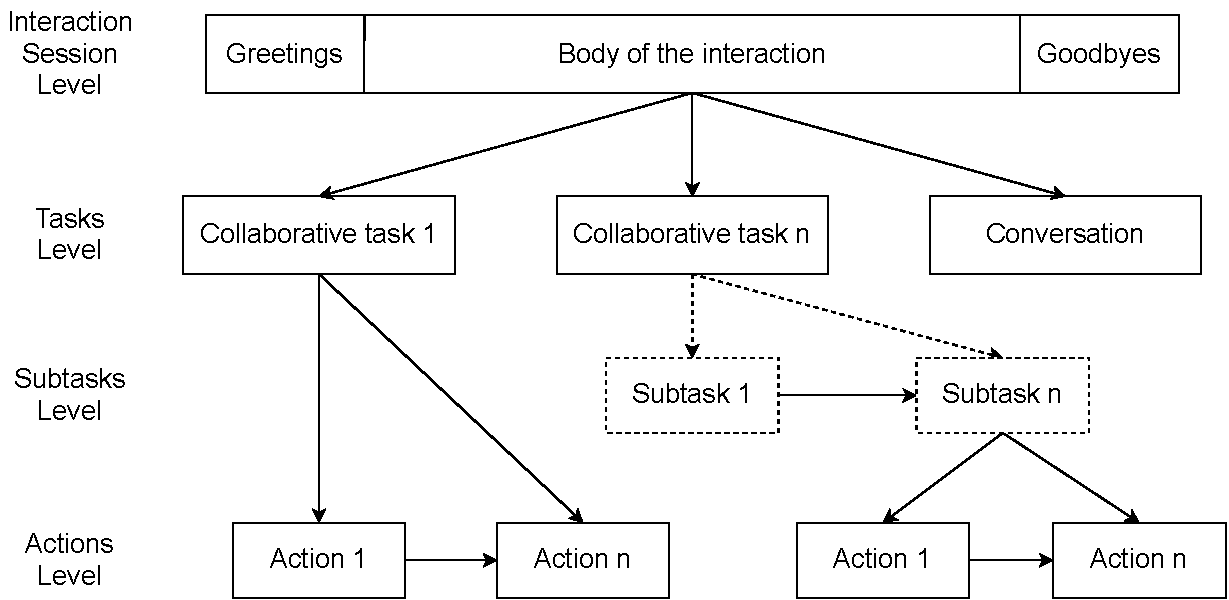
\includegraphics[width=\linewidth]{figures/chapter2/session_interaction.pdf}
	\caption{The hierarchical structure of an interaction session. The highest level is the interaction session. The second level is composed of the tasks. They are included in the body of interaction of the interaction session and, two types of tasks are considered and may overlap, collaborative and conversational tasks. With this representation, a task can be recursively refined as subtasks until reaching the last level, the actions level, which is considered as atomic. Subtasks are not considered as a ``real'' level of the interaction session, specially to evaluate the QoI, as it may exist or not according to the task.}
	\label{fig:levels}
\end{figure}


\subsection{Representation of a Human-Robot Interaction Session}
We define an \textbf{interaction session} as the period during which the robot and a human interact together and are engaged. It is divided in three parts, following the structure proposed by Robinson~\cite{robinson_overall_2012} as presented in Section~\ref{chap1:sec:soc_inter}: the greetings, the body of the interaction and the goodbyes. First, \textit{the greetings} corresponds to the period where an agent starts an interaction by initiating it with another agent. The interaction session lasts as long as the interactants are maintaining the interaction through conversation and collaborative tasks performance which corresponds to the \textit{body of interaction}. Finally it ends when at least one of the interactants is disengaged, either by abruptly ending the interaction or by closing the interaction as described by Schegloff and Sacks~\cite{schegloff_1973_opening}, it corresponds to ``the goodbyes''. For example, for an entertainment robot in a mall, an \textit{interaction session} starts when a person signals to the robot that they want to engaged, by greeting it or by approaching it and looking at it. The body of interaction is composed of conversation and eventually direction-giving tasks and, the session lasts until the person says goodbye or leaves. This is the nominal case and, the duty of the robot is to contribute to maintain the session alive until the human decide to close it. However, in some (extreme) cases, the robot might decide to close the interaction by itself.

Social interactions and collaborative tasks involve engagement. There is no unique definition of what it means to be engaged. We chose one that is frequently used and has been proposed by Sidner and Lee~\cite{sidner_2003_engagement}\todo{lien avec commitment chap 1}: ``Engagement is the process by which two (or more) participants establish, maintain and end their perceived connection during interactions they jointly undertake''. The robot must be able to exhibit its engagement and disengagement and also to assess them with respect to its human partner.
We defined three states for the body of interaction, corresponding to what is happening during the latter: conversation (\ie a social chit-chat or a goal negotiation, without any physical action performed except communicative gestures), collaborative task (\ie both agents executing actions in order to achieve a shared goal) or idle phases (\ie the agents are not chatting or performing a collaborative task together but remain engaged in the interaction session, it happens in-between active interaction phases). For each of these three states, the way to exhibit the engagement varies (\eg in a conversation, an agent looking at their partner displays their engagement; during a task, an agent correctly performing their action is a way to demonstrate their engagement). That is why there is a need to define what behavior the robot has to exhibit in each state and what behavior it should expect from the human in each state, as these behaviors are usually very specific (\eg in a direction-giving task, the robot keeps its head oriented toward its partner's face to demonstrate its engagement in conversation and idle contexts and when it gives a direction it expects the human to look at the direction it is showing; in a stack task, when the robot gives an instruction it expects the human to take a given cube).


\subsection{Collaborative Tasks, Substasks and Actions}
\textbf{\textit{Tasks}} compose the body of the interaction of an interaction session as shown in Fig.~\ref{fig:levels}. We distinguish conversation (\ie agents engage in dialogue to exchange ideas, to ask questions, and to resolve differences) from collaborative tasks (\ie agents work as partners, collaborating to perform tasks and to achieve common goals). We will not develop more on conversation since it is not the main focus of this paper, assessing the QoI of social dialog being another work.

In collaborative tasks, the robot and the human are committed to achieve a goal together, involving joint actions and shared plans~\cite{grosz_1996_collaborative}.  When a human and a robot perform a task together, as described by Bauer \textit{et al}.~\cite{bauer_2008_collab}, we could say that the robot has the intent to help the human, so the human's intention becomes its own intention. Then, they have the joint intention to reach a common goal and, as shown by Michael and Salice~\cite{michael_2017_commitment}, they have a commitment to the joint activity, leading to perform joint actions. Therefore, during its evaluation and decision-making processes, the robot has to take into account that the human and itself should remain engaged all along an interaction session for the tasks to be successful and both have to manage and contribute to maintain expectations about what the other is doing. 

The elements composing a \textit{task} are: a goal, a plan and involved agents. A plan is needed to realize a goal. There are many ways to generate a plan. But no matter the way (using a planner to anticipate execution or relying on a reactive planning scheme), a plan is a sequence of \textbf{\textit{subtasks}} which are sequences of actions -- \textit{subtasks} are not considered as a ``real'' level of the interaction session, specially to evaluate the QoI, as it may exist or not according to the task.
%-- sometimes it is not necessary to have an additional abstraction level, in this case a plan is directly composed of actions, with no subtasks. 

\textbf{\textit{Actions}} are the elementary items of tasks manipulated by the high-level robot supervision controller. They cannot be decomposed further by it (\eg placement and motion planning are achieved by a lower control system not described here). It is usual to describe an action with its preconditions, its effects and, the agents and entities implied in its execution (\eg in plans written in PDDL (Planning Domain Definition Language)~\cite{ghallab_98_pddl}). We add to this description the notion of expected reactions (which can themselves be actions) from the other agents once the action is executed.

In our model, an agent (human or robot) is a contributor to the task and has a mental state as described by Devin \textit{et al}.~\cite{devin_2016_implemented}. The mental state is a set of facts representing, from the agent point of view, the current world state, the state of the goal and the current task state. Since we are interested here by the robot situation assessment and decisional processes, the mental state of the human is built and managed by the robot as an estimation of the beliefs of the human~\cite{milliez_2014_framework, hiatt_2017_modeling,tabrez_2020}.

\section{A BDI Framework as a Base of JAHRVIS Architecture}


\subsection{The Choice of the Framework}
Restart from scratch or base oneself work on an existing software? This is the question which has been studied at the beginning of this thesis work about the implementation of the supervision software. It was possible 
\begin{enumerate*}[label={(\arabic*)}]
	\item to develop the wanted features using the code\footnote{\url{https://github.com/laas/supervisor}} of the previous PhD student working on the supervision, Sandra Devin,\label{chap2:list:sandra}
	\item to choose among existing software dedicated to decision and execution for Human-Robot Interaction,\label{chap2:list:soft_hri}
	\item to choose among existing software dedicated to decision and execution for robotic platforms, and\label{chap2:list:robot}
	\item to develop a new software from scratch.\label{chap2:list:new}
\end{enumerate*}

The obvious drawback of \ref{chap2:list:new} is that it takes a lot of time to start a new software from scratch and that it often leads to reinvent the wheel. Then, first we looked at existing solutions. Concerning the possibility \ref{chap2:list:sandra}, she had developed interested features but the code is not modular and it was difficult to add new features or to do modification of the existing ones without breaking everything. Thus, there was the solutions \ref{chap2:list:soft_hri} and \ref{chap2:list:robot} left. When looking for existing software to manage human-robot interactions, we could find any open-source one with a minimum of features, documentation and not entirely dedicated to a given task. Therefore, we turned ourselves toward robotic frameworks. We compared existing open-source decision-making and execution software for robots. To cite a few, there is the PetriNetPlans library introduced by Ziparo \etal~\cite{ziparo_2011_petri} which is a framework for planning and execution. Beetz \etal{} developed CRAM, a software implementing reasoning mechanisms that can infer control decisions~\cite{beetz_2010_cram}. A framework to implement hierarchical state machines is available among ROS libraries, SMACH\footnote{\url{http://wiki.ros.org/smach}}, defined as ``task-level architecture for rapidly creating complex robot behavior''. Finally, there are several implementations of the BDI model presented in Section~\ref{chap1:sec:archi} such as JAM~\cite{huber_1999_jam}, Jadex~\cite{braudach_2005_jadex}, SPARK~\cite{morley_2004_spark}, dMARS~\cite{dinverno_1998_formal}, OpenPRS~\cite{ingrand_1996_prs} or Jason~\cite{bordini_2007_jason}. 

Our choice went to SMACH because its compatibility with ROS and its facility to be used. However, after having built a first prototype with it, we realized the limitations of the framework, as it became more and more difficult to program complex robot behaviors, state machine were not enough powerful. Thus, we returned to the drawing board, minus one option. After a comparison considering potential compatibility with ROS, possible integration with the other software of our architecture, availability of documentation, users' feedbacks, maintenance, and possibility of code modifications, our choice went to Jason designed by Bordini \etal~\cite{bordini_2007_jason} which is a Java interpreter of AgentSpeak created by Rao~\cite{rao_1996_agentspeak}. It has the advantage to be a BDI (Beliefs, Desires, Intentions) (see Section~\ref{chap1:subsec:archi}) agent-oriented framework, fitting with our architecture. BDI frameworks are primarily focused on practical reasoning, \ie the process of deciding, step by step, which action to perform to reach a goal. It allows more modularity than state machines to handle contingencies and events. It also facilitates reasoning on agents' -- humans and robot -- beliefs. We chose this framework among the BDI ones and not another because it is implemented in Java and thus was compatible with rosjava\footnote{\url{https://github.com/rosjava/rosjava_core}} (\ie ROS implementation in Java), it is still developed and maintained, it is well documented (theoretically~\cite{bordini_2007_jason} and implement-ally\footnote{\url{http://jason.sourceforge.net/api/}}) which allows source code understanding and modifications, and there is a mailing list for users and its archives available\footnote{\url{https://sourceforge.net/p/jason/mailman/jason-users/}}.

\subsection{Programming with Jason}\label{chap2:subsec:jason}
As said above, Jason is a BDI-based framework, allowing what is called \textit{agent-oriented programming}. Originally designed for multi-robot programming, it can be used for other purposes such as our. How does it work?

We explained in Section~\ref{chap1:subsec:archi} that there were three main concepts to retain from the BDI model: beliefs, desires and intentions. Well, Jason's purpose is to program agents. Thus, each agent has a beliefs, desires and intentions. The beliefs are what it perceives, acquires from other agents and computes. They can produce desires, \ie states of affairs the agent wants to achieve. Then, the agent deliberates on its desires and chose to commit to some of them, \ie the chosen desires become intentions. To satisfy its intentions, the agent executes plans leading to actions. 

The programming of the behavior of an agent is in the AgentSpeakLanguage (ASL). The program is designed by a user, a programmer. A program contains, among other things, plans. These plans have actions. An action is described by a Java program, written by the Jason's user. Then, to run, a program uses the decision loop, the \textit{reasoning cycle}, integrated to Jason. It is possible to customize some functions of the reasoning cycle by overloading or adding Java functions of the agent's constructors, belief base and reasoning cycle. 

\subsubsection{Agents} In the ASL program of an agent, it is possible to see plans, beliefs, achievement goal (desire) and test goal. First, let's see a very simple example of program with the agent Bob\footnote{\url{http://jason.sourceforge.net/mini-tutorial/hello-bdi/}}, presented in Listing~\ref{chap2:lst:bob}. Bob has one initial (\ie given by the programmer, not acquired by perception) belief which is |happy(bob)|. A belief is a property, here |happy|, which can have whatever number of arguments (including zero), here |bob|. Then, he has one initial desire, or achievement goal, which is recognizable by |!|. And finally, he has a the plan allowing to achieve the desire |say(hello)|. A plan is triggered by an event, here |+!say(X)| (\ie the event is that the goal |say(hello)| has been added), has a context (\ie a precondition), here |happy(bob)| and has a body which contains the actions to execute, here |.print(X)| (\ie |X| is a non-initiated variable at first, that will take the value |hello| when Bob will transform his desire into an intention). If we remove the initial belief |happy(bob)| from the first line, as the program is written and considering that Bob is the only agent, he cannot print hello, as the precondition of the plan will not be true.

\begin{lstlisting}[caption={ASL program of Bob, a Jason agent}, label={chap2:lst:bob}]
happy(bob).	\\belief

!say(hello).	\\achievement goal

+!say(X) : happy(bob) <- .print(X).		\\plan
\end{lstlisting} 

In another example, illustrated by Listing~\ref{chap2:lst:bobalice}, Bob has no initial belief nor initial goal. He has plans for two events: starting to believe he is happy and having the goal to say hello. We can see that there is also a program for another agent, Alice. She has an initial goal, her, which is to inform bob that he is happy. Therefore, we can see that an agent can add a belief in another agent's belief base. When Bob gets the information that he is happy, this triggers his first plan, creating for him the goal |!say(hello)|. As Bob does not believe that today is Monday, he can trigger his second plan to say hello. In this plan, there a three elements: a print action, a wait action and the addition of a new goal. And thus, here, we are in the presence of a recursive plan which never ends. 

\begin{lstlisting}[caption={ASL programs of Bob and Alice, two Jason agent}, label={chap2:lst:bobalice}]
\\bob.asl
+happy(bob) : true <- !say(hello).

+!say(X) : not today(monday) <- 
.print(X); 
.wait(500); 
!say(X).

\\alice.asl
!inform.

+!inform : true <- .send(bob,tell,happy(bob)).
\end{lstlisting} 

\subsubsection{Actions} To give an idea of what looks like the Java program of an action, here is an example of a Java function for the action |.print| in Listing~\ref{chap2:lst:print}.

\begin{lstlisting}[caption={.print action}, label={chap2:lst:print}, language=Java]
public class print extends DefaultInternalAction {
	@Override
	public Object execute(TransitionSystem ts, Unifier un, Term[] args) throws Exception {
		String sout = argsToString(args);
		System.out.print(sout.toString() + "\n");
	}
	return true;
	}
}
\end{lstlisting} 

In Jason, there are two types of action: \textit{environment actions} and \textit{internal actions}. \textit{Environment actions} allow an agent to act within its environment whereas \textit{internal actions} are designed to be run internally within an agent such as the print action.

We have seen what looks like the program of Jason agent. Now, we are going to see how it is run by the Jason interpreter.


\subsubsection{Reasoning cycle} Each agent has what has been coined a \textit{reasoning cycle}, composed of 10 steps. It resembles a decision loop, running each step one by one and starting again at the first one. The steps 1 to 4 are dedicated to the belief update of the agent. The steps 5 to 10 describe the interpretation of the ASL program. In these latter, an event is selected, as well as a plan corresponding to this event and then the first formula (\eg an action or a goal) of the plan is executed. The steps are the following ones, in this order:
\begin{enumerate}
	\item Perceiving the Environment: Each agent has a Java function called |perceive|. This function can retrieve data from a simulated environment or be customized by the programmer to get actual perception data. The function output a list of beliefs (\eg |<isOn(box1,table)[source(percept)]|, |color(box1,red)[source(percept)]>|).
	\item Updating the Belief Base: The agent's belief base is updated with the perception data. Each change in the belief base generates an event (\eg |+color(box1,red)[source(percept)]| and if later the color of the box is not perceived anymore, it will be |-color(box1,red)[source(percept)]|).\label{chap2:list:update_bb}
	\item Receiving Communication from Other Agents: It checks if an agent received a message from another agent such as the message Bob received from Alice in Listing~\ref{chap2:lst:bobalice}. A message can be a belief, a plan, a goal or a questioning on a given belief.
	\item Selecting ‘Socially Acceptable’ Messages: It is a function the programmer should customize. It allows that an agent refuses messages or types of message from some given agents.
	\item Selecting an Event: Events are either perceived changes in the environment or changes in the agent's own goals. There is a queue of events and at each reasoning cycle only one is selected to be handled. The default method to select it is a FIFO but as every function of the reasoning cycle, it can be customized. 
	\item Retrieving all Relevant Plans: From the selected event, it tries to find all the relevant plans for this event, in the plan library, \ie the plans written by the programmer in ASL. The function tries to find the plans that can be \textit{unified} with event, \ie the ones with their left part (the trigger) match the event. For example, if the selected event is |+color(box1,red)[source(percept)]| and in the plan library there are these six plans:
\begin{lstlisting}[style=inline]
+position(Object,Coords) : true <- .print(Coords).
+color(Object,red) : true <- .print(nice).
+color(Object,red)[source(self)] : true <- .print(nice).
+color(box1,Color) : true <- .print(nice).
+color(Object,Color) : false <- .print(Color).
+color(Object,blue) : true <- .print(so-so).
\end{lstlisting}
	then there are three relevant plans:
\begin{lstlisting}[style=inline]
+color(Object,red) : true <- .print(nice).
+color(box1,Color) : true <- .print(nice).
+color(Object,Colour) : false <- .print(Colour).
\end{lstlisting}
	\item Determining the Applicable Plans: It takes the list of relevant plans and sees which ones are applicable. To do so, it looks at the context (the preconditions) of the plans. The context can be beliefs, prolog-like rules, internal actions, logical expressions or booleans. If we look at the example of the previous step, there were three relevant plans. Their contexts are simple booleans. Two of them are true, the other one is false, thus the two first plans are applicable.
	\item Selecting One Applicable Plan: It takes the list of applicable plans and select the one that will be elected to become an intention, \ie to be executed. As usual, this is a customizable function for which the default behavior is to take the first plan in the order of the plan library, \ie in the order written by the programmer. Still with the same example, thus, the one plan to be selected is the first one, |+color(Object,red) : true <- .print(nice).| If the event was external, \ie from perception, it creates a new intention, adding it to the set of intentions. Then, the agent has a new \textit{focus of attention}. If the event was internal, \eg a belief addition inside a plan, then the selected plan is added on the top of the existing intention. 
	\item Selecting an Intention for Further Execution: As seen in the previous step, an agent can have more than one intention in the set of intentions, each representing a different focus of attention. Then, at this step is chosen the intention of which the formula will be executed. The default function choses the first intention of the list. After execution of the formula, the intention will go at the end of the intentions list.
	\item Executing One Step of an Intention: The first formula of the selected intention is executed (this number is also customizable and the programmer can choose that an agent execute more than once formula in the same reasoning cycle). It can be an internal action, an environment action, a goal, a belief addition or deletion and two other types that will not be developed here. 
\end{enumerate}

Therefore, each agent has a reasoning cycle running repeatedly.

\subsection{Jason Integration with ROS}
The robotic architecture presented in Section~\ref{chap2:sec:rob_archi} uses the ROS framework\cite{quigley_2009_ros} to enable communication between its components. Thus, to be able to build a supervision software based on Jason, we needed to interface it with ROS as well. At the time, there was no available bridge between Jason and ROS, Jason being extensively used in simulation contexts. Thus, we developed our own -- and at about the same moment, the Jason's developers started to develop theirs~\cite{silva_2020_embedded} (what we realized a bit later), both using rosjava. We tackled the problem in very different ways. A user of their implementation only needs to fill one perception (topics) and one action (topics/services) manifests to link the system with ROS and then implement their agent in ASL. Thus, it is quite easy to use. However, it seems to have backlashes. Therefore, action requests are directly sent from ASL to the hardware controller, with no possibility of Java processing. Moreover, action status/result can only be boolean which is not enough for a system like ours needing to perform service queries of data to the external Knowledge Base for example. Finally, there is no bridge with action servers which are often use for motion planers for example. 

\begin{figure}[!ht]
	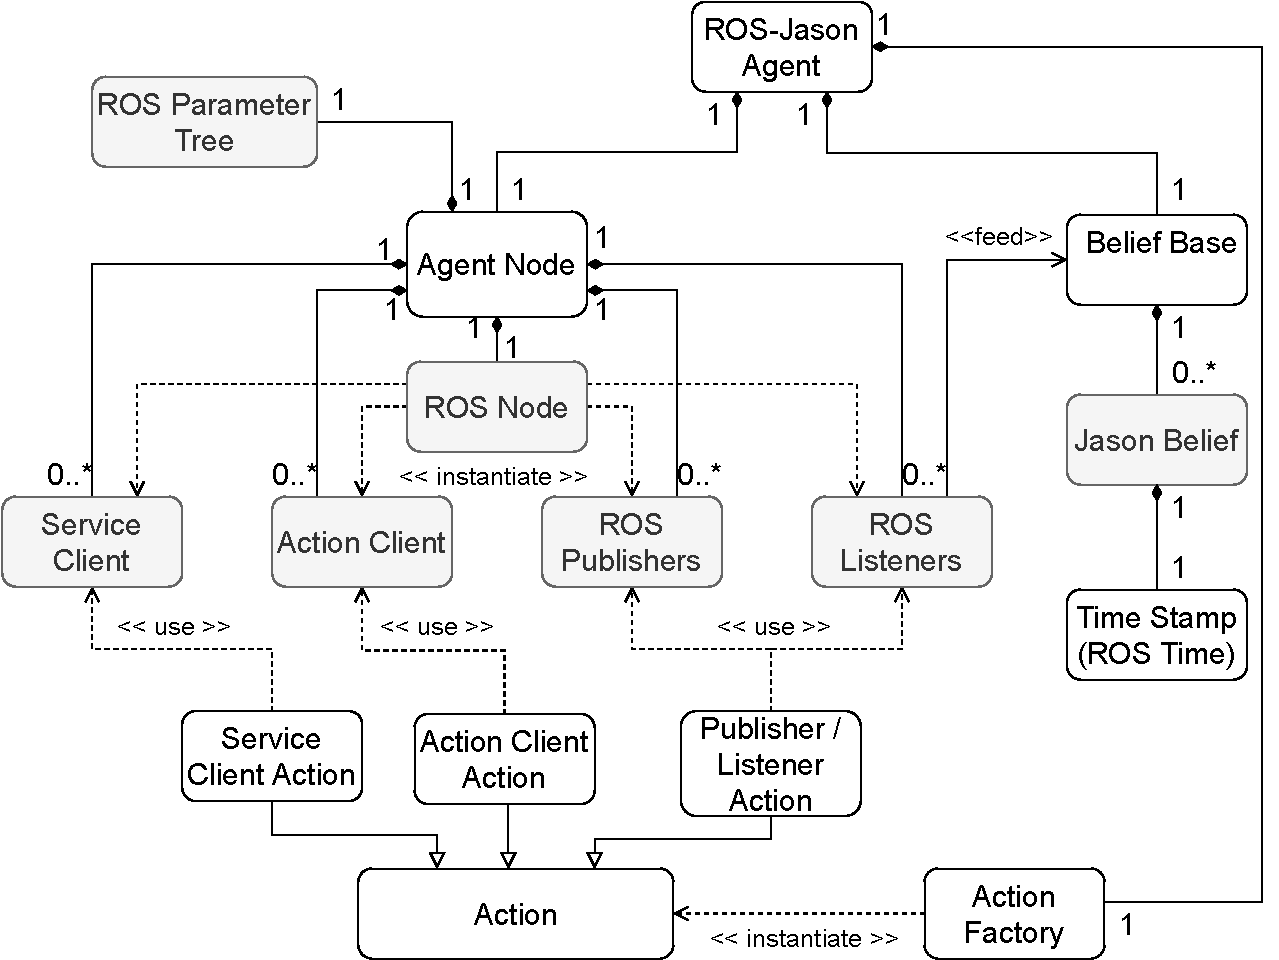
\includegraphics[width=\linewidth]{figures/chapter2/RJS_diagram.pdf}
	\caption{Simplified Java class diagram of our ROS-Jason implementation. In white are our customized classes and in grey the native ROS and Jason classes.}
	\label{chap2:fig:rjs}
\end{figure}

A simplified Java class diagram of our  implementation\footnote{\url{https://github.com/amdia/rjs}} is presented in Figure~\ref{chap2:fig:rjs}. We defined for each Jason agent a customized Java class (\acrfull{rja} on the figure) which has an Agent Node, an action factory and a belief base where all beliefs are time stamped with the roscore time. 

An Agent Node has an attribute, the ROS Parameter Tree, allowing to load YAML parameters from files in which, among other things, are written services, topics and action servers info, as shown in Listing~\ref{chap2:lst:ros-jason}, a bit similarly to the manifests of~\cite{silva_2020_embedded}. From these parameters, the Agent Node can automatically instantiate all the needed ROS components through its ROS node. 

The Belief Base can receive perception updates through ROS topic listeners. Moreover, we customized\footnote{This modification of the belief update function is not part of our ROS-Jason implementation but is on top of it, in the \acrshort{jahrvis} implementation which relies on ROS-Jason.} the belief update function (step~\ref{chap2:list:update_bb} of the reasoning cycle) so percepts are not elements that when perceived at time T are added to the belief base and disappearing when not perceived anymore at time T+1. There are updates (additions and deletions) from the external Knowledge Base, in this way, it limits the number of message exchanges, \ie instead of receiving every 500 ms during 10 seconds that the agent perceives |cube_1|, it receives for example an addition at t=18s and a deletion at t=28s. 

For each belief added in the belief base, from perception or internal computation, is added a time stamp from the current ROS time. It is useful for the computation of the Quality of Interaction presented in Section~\ref{chap2:sec:qoi} and for debugging.

An \acrshort{rja} has a Action Factory -- abstract in the ROS-Jason framework and instantiated in \acrshort{jahrvis} -- containing the list of environment actions it can perform -- in the case of our architecture, not all actions of this type are for the robot to act on its environment, sometimes there are queries to other components of the architecture. The Action Factory instantiates the Action called through the ASL program at execution time. An Action can either be based on either a ROS service client, or an ROS action client or a ROS publisher for the request and a ROS listener for the result. 

\begin{lstlisting}[caption={Example of service, topic and action server definitions in a YAML file.}, label={chap2:lst:ros-jason}]
services:
	onto_individual: 
		name: /ontologenius/individual/robot
		type: ontologenius/OntologeniusService
	onto_class: 
		name: /ontologenius/class/robot
		type: ontologenius/OntologeniusService
topics:
	mementar_occasions: 
		name: /mementar/occasions/robot
		type: mementar/MementarOccasion
		function: sub
	plan_request:
		name: /planner/request_new_plan
		type: planner_msgs/PlanRequest
		function: pub
action_servers:
	plan_motion: /pr2_tasks_node/plan
	execute_motion: /pr2_tasks_node/execute
\end{lstlisting}


\section{The Architecture of JAHRVIS}
The \acrfull{jahrvis} is implemented on top of our ROS-Jason framework. During the design of \acrshort{jahrvis}, we identified seven high-level features we needed and implemented their associated processes, based on the objectives presented in Section~\ref{chap2:sec:sup_features}\footnote{The design of \acrshort{jahrvis} was an iterative work, indeed the first version being the supervisor implemented for the task described in Chapter~\ref{chapter:chap3}, the second one was the supervisor of the task described in Chapter~\ref{chapter:chap4} and the final one was the supervisor of the task described in Chapter~\ref{chapter:chap5}}\todo{derniere tache existera???}. We present \acrshort{jahrvis} architecture in Figure~\ref{chap2:fig:sup_overview}. 

\begin{figure}[!ht]
	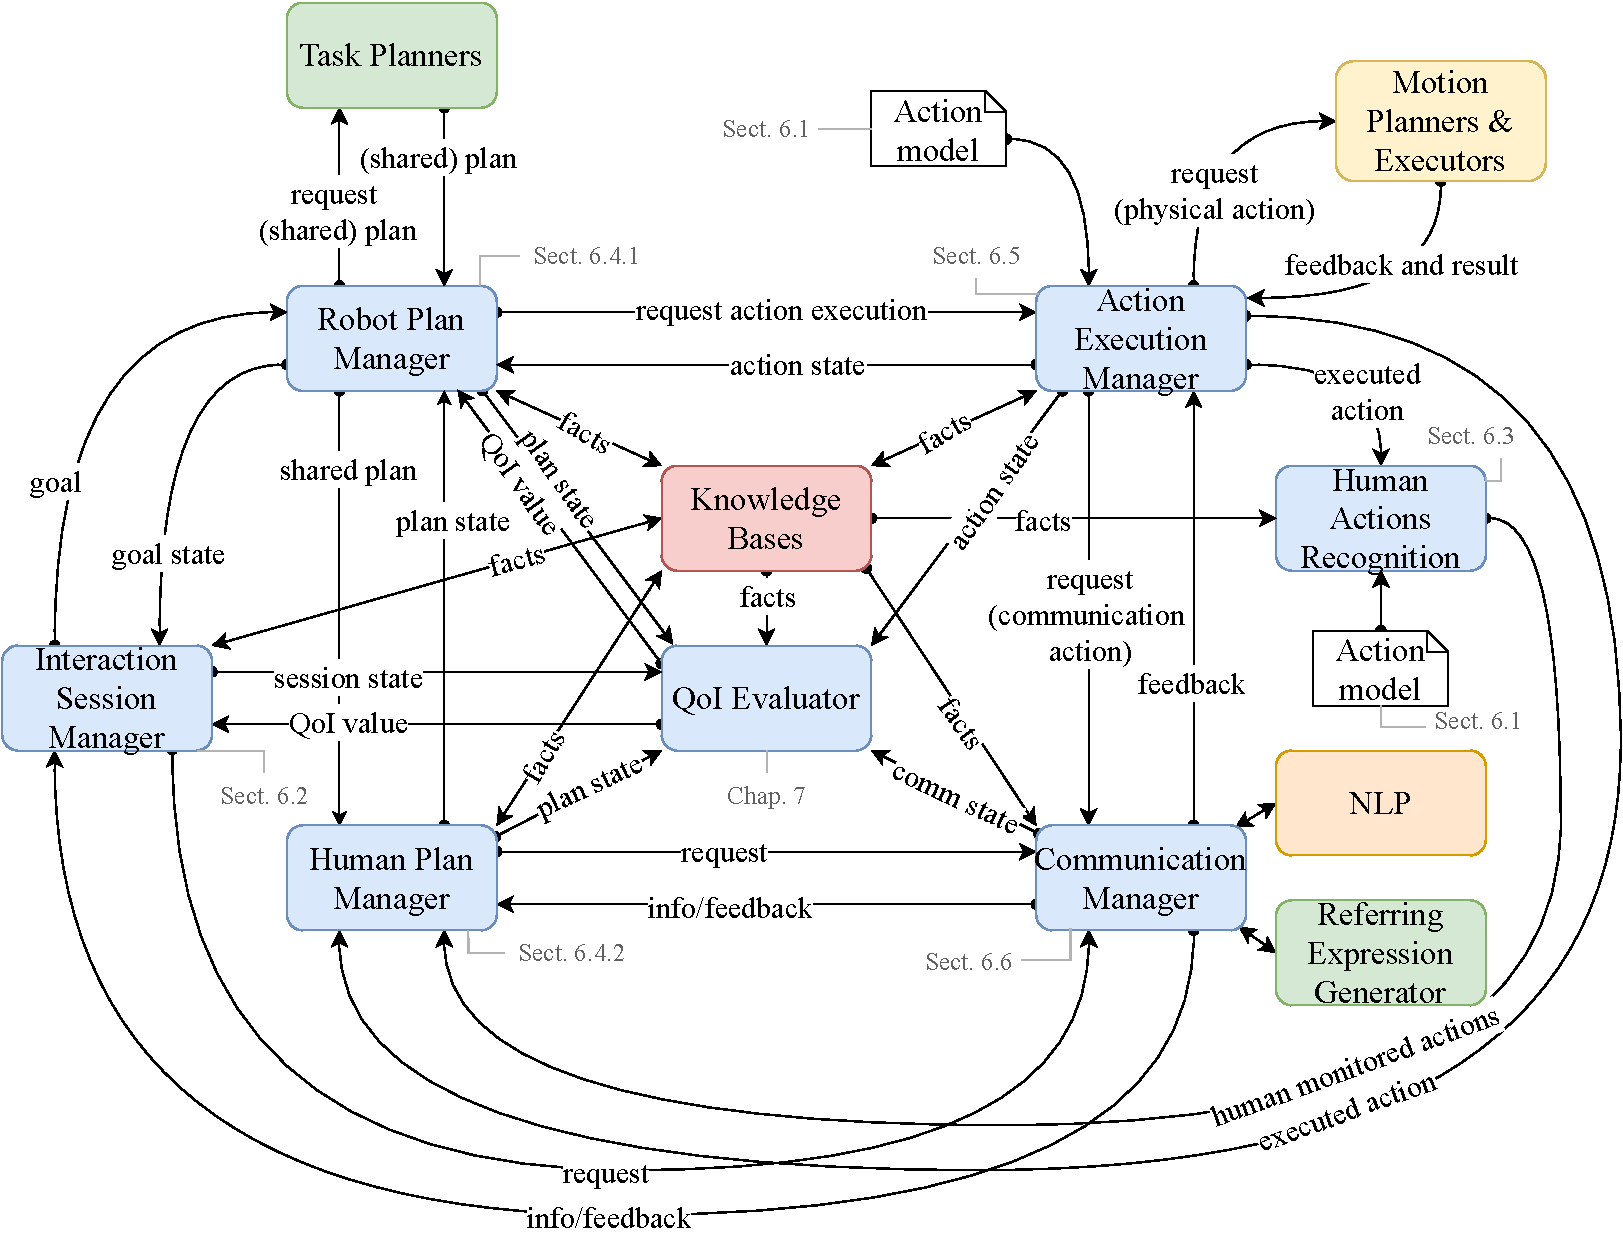
\includegraphics[width=\linewidth]{figures/chapter2/supervisor_modules.pdf}
	\caption{The \acrshort{jahrvis} processes (in blue) and their interactions between themselves and with the other components of the architecture.}
	\label{chap2:fig:sup_overview}
\end{figure}

For each processes (in blue in Figure~\ref{chap2:fig:sup_overview}), we implemented an \acrshort{rja}, with the wanted behavior coded in ASL and the needed customizations added in Java. Thus, internal communications between the \acrshort{jahrvis} processes, and so \acrshort{rja}s, use Jason messages (see Section~\ref{chap2:subsec:jason}). External communication with the other components of the robotic architecture is based on either ROS messages, services or action clients.

Not all \acrshort{rja}s are active at each level of interaction defined in Section~\ref{chap2:sec:levels}. Indeed, as its name suggests, the \textit{Interaction Session Manager} handles interaction sessions. The \textit{Robot} and \textit{Human Plan Managers} handle the task level. And, the \textit{Action Execution Manager} and the \textit{\acrlong{ham}} are in charge of the action level. The \textit{QoI Evaluator} and the \textit{Communication Manager} are active at all levels. We can also make the distinction between the component dedicated to the assessment of the quality of interaction, \ie the QoI Evaluator, and the components dedicated to the decision-making and control, \ie all the components except the QoI Evaluator.


\section{A robot controlling its contribution to a human-robot joint action}\label{chap2:sec:control}

The objective of this section is to present the \acrshort{jahrvis} processes involved in the decision-making and the control of the robot when jointly interacting with a human. First, we present the knowledge representations used, then the Interaction Session Manager, the Human Actions Monitoring, the Shared Plans Handling composed of two processes, one for the robot and one for the human, the Action Execution Manager, and finally the Communication Manager.

\subsection{Knowledge Representations and Management}\label{chap2:subsec:know}
As shown in Section~\ref{chap1:subsubsec:shared_rep} and Section~\ref{chap1:subsubsec:common_g}, when involved in joint actions, humans have shared representations of tasks, actions, goals and have a common ground. Thus, it is important that the robot has such internal representations.

During an interaction, \acrshort{jahrvis} processes use knowledge bases (KB) of two types: external and internal ones. The external knowledge bases with which we interfaced \acrshort{jahrvis} are Ontologenius\footnote{\url{https://github.com/sarthou/ontologenius/}}~\cite{sarthou_2019_ontologenius} for the semantic knowledge and Mementar\footnote{\url{https://github.com/sarthou/mementar}} for the episodic one. They have been developed by Guillaume Sarthou with whom we collaborated closely. Then, each \acrshort{rja} has its own knowledge base that we call belief base in Jason vocabulary. It is used for knowledge which serves to \acrshort{jahrvis} internal computations only.

Ontologenius allows to store common-sense knowledge (\eg a cube is an object), knowledge about the environment (\eg object\_1245 is a Cube and is on top of table\_2) and knowledge about activities grounded in space and time (\eg object\_1245 has been put on the table\_2 by robot (action ID 475)). Mementar allows to store facts and actions in a timeline (\eg action ID 475 started at 3286 seconds and was over at 3290 seconds). As stated in Section~\ref{chap2:sec:rob_archi}, it receives and stores facts about the current state from the Situation Assessment component. It reasons on it (\eg after receiving \fact{isOnTof}{cube\_2}{table\_1} and it computes \fact{isUnder}{table\_1}{cube\_2}). 

To access to the knowledge stored in Ontologenius, \acrshort{jahrvis} can make a request to know if a given fact exists or ask an information about a class, a property or an object instantiation. Another way is to subscribe to updates (addition or deletion) for a given fact. It is useful to keep updates about the environment and avoid to be snowed under too much data (\eg to monitor human place actions, \acrshort{jahrvis} needs \textit{isOnTopOf} but not \textit{isUnder} so \acrlong{ham} can subscribe to updates about this first fact). It is possible to either specify the class or individual of the subjects/objects that should be concerned by the subscription, or to receive every facts (\eg it can subscribe to receive additions of the human looking at the robot |[add]human_0$\lvert$isLookingAt$\lvert$robot| or to receive all updates about every objects that the human looks at |[?]human_0$\lvert$isLookingAt$\lvert$?|).

\subsubsection{Action Representations}
Action representations allow the robot to recognize actions, to execute actions, to monitor the human monitoring its actions and to communicate about them. We defined three of them. We chose to have one stored in Ontologenius to benefit from the reasoning features and to have the two others written in an ASL file to benefit from Jason reasoning features.

\paragraph{External Representation}
For the needs of \acrshort{jahrvis}, we represented actions, their verbal labels and their effects in a semantic \acrshort{kb} in the form of an ontology\footnote{An ontology is a way to represent knowledge} managed by Ontologenius. We show in Figure~\ref{chap2:fig:class_actions} a representation of some actions we stored in Ontologenius using the Web Ontology Language (OWL) (see Listing~\ref{chap2:lst:classes}) and in Figure~\ref{chap2:fig:class_effects} a representation of possible action effects.

\begin{lstlisting}[style=OwlTurtle, label={chap2:lst:classes}, caption={Description of ontology classes in the OWL language using the Turle syntax.} ]
:PhysicalAction	rdf:type owl:Class ;
				rdfs:subClassOf :HtnAction .

:ScanAction	rdf:type owl:Class ;
			rdfs:subClassOf :PhysicalAction ;
			htn_actions:hasEffect :IsScannedEffect ;
			rdfs:label ``{Agent} @Scan {Pickable}'' .

\end{lstlisting}

One of the advantages of using action model stored in Ontologenius is the class inheritance. It allows to define properties for one class that will be transmitted to its child classes (\eg if it exists multiple class representing a drop action, let's say |human_drop_cube| and |robot_drop_cube|, both inherit from the properties of |DropAction| such as the label used for the action verbalization). Another advantage is to be able to link classes through properties and to easily query the \acrshort{kb} about it (\eg what are the effects of the |PickAction| and then what types of effects are they?).

\begin{figure}[!ht]
	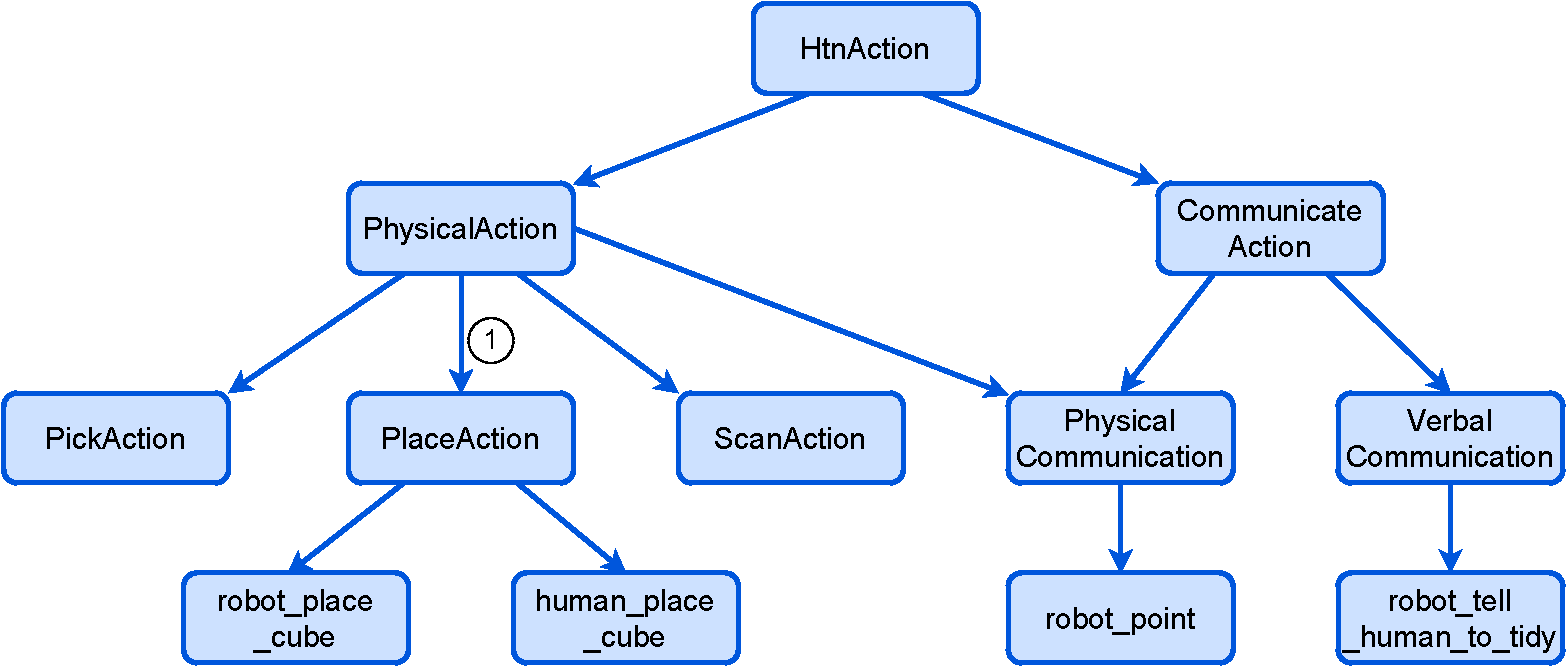
\includegraphics[width=\linewidth]{figures/chapter2/class_actions.pdf}
	\caption{The representation of an extract of the ontology class hierarchy graph of \acrshort{htn} actions. Taking the class PhysicalAction, the middle bottom arrow has to be read	as \textit{``A DropAction is a kind of PhysicalAction''}.}
	\label{chap2:fig:class_actions}
\end{figure}

\begin{figure}[!ht]
	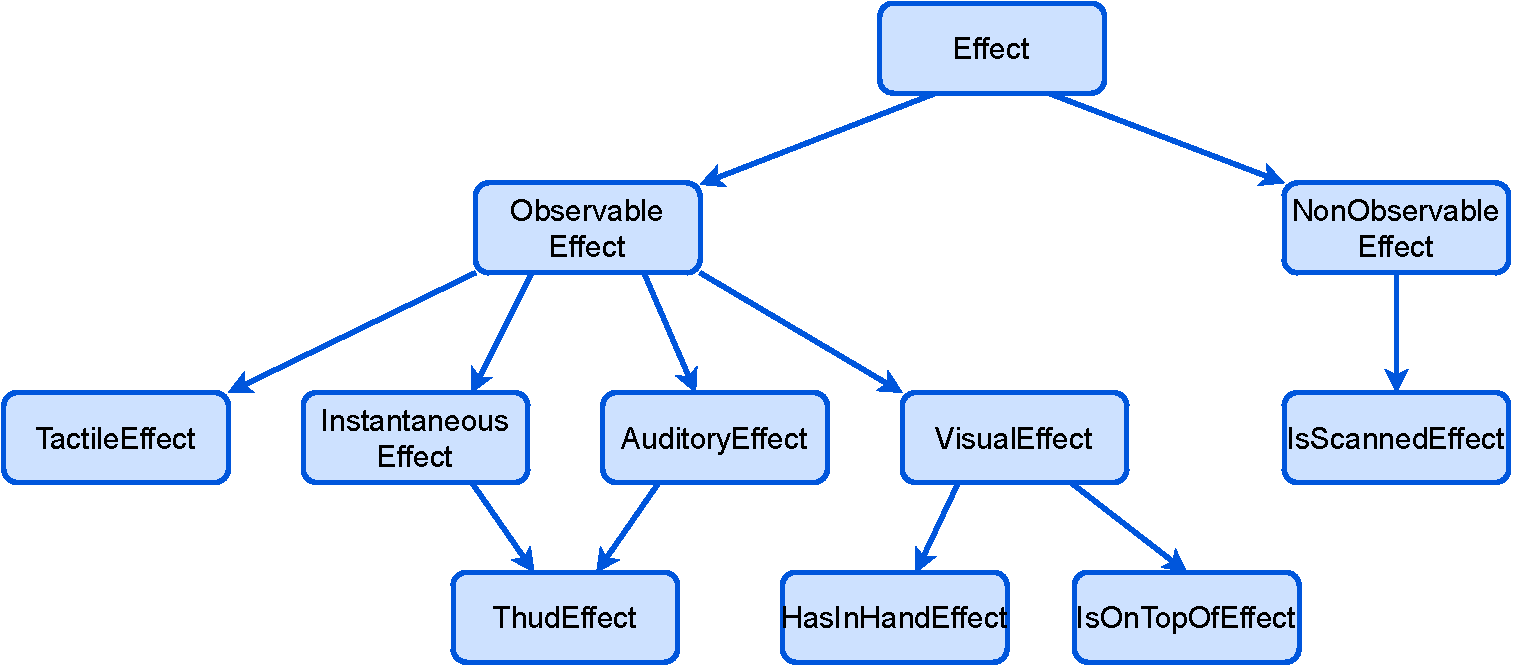
\includegraphics[width=\linewidth]{figures/chapter2/class_effects.pdf}
	\caption{The representation of an extract of the ontology class hierarchy graph of action effects. Taking the class ThudEffect, the top arrows indicate that ThudEffect is and an InstantaneousEffect and an AuditoryEffect.}
	\label{chap2:fig:class_effects}
\end{figure}

As we know, when an agent perform an action, the other agent may monitor it, in order to follow the task progress and to know when the action is over. A way to know that an action is over is to check if the action effects exist or not in the current worldstate. However, effects may be perceived differently according to the agent type as humans and robots does not have the same perception modalities (and even in one given type it can differ). In Figure~\ref{chap2:fig:class_effects}, we represented a possible way to model and classify action effects. And so, because Ontologenius is designed for \acrshort{hri}, it is possible to have different representations for robot agents and human agents. We present now a use case with its illustration in Figure~\ref{chap2:fig:kettle}. An agent may have to perform |HeatWaterInKettleAction|. If it is performed by the human, the robot has to monitor the action effects to know if the action is over or not. However, a robot is not able to observe that a kettle has finished to boil water, thus the action has a non-observable effect for the robot. Then, probably the robot will ask the human if the action is over or will see that the human performs its next action of the plan. Now, if we place ourselves in the case where the robot is the one performing the action -- with a smart kettle --, it wants to check if the human could be aware of the action end (because if they are not aware, it needs to communicate about it). The criteria \acrshort{jahrvis} takes into account is, was the effect observable by the human partner? To answer this question, it first needs to know what the observable effects of |HeatWaterInKettleAction| for the human (if there are). Then, it can query the human's belief base in Ontologenius and get the knowledge that for them, the effect of |HeatWaterInKettleAction| belongs to the class |ThudEffect| (when the kettle stops, it produces a thud) and |TactileEffect| (when the kettle boils water, it becomes hot).
	
\begin{figure}[!ht]
	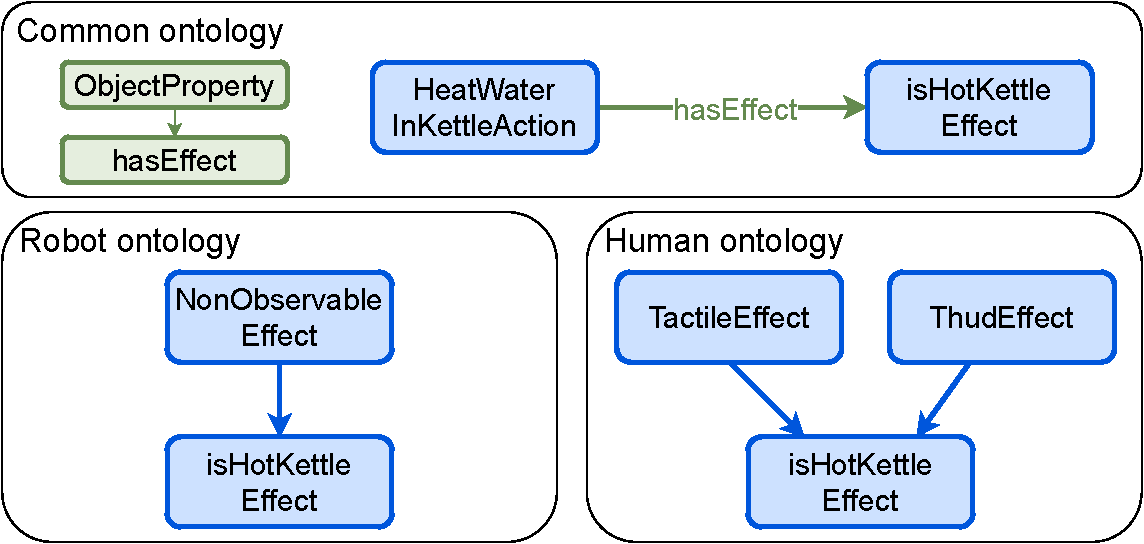
\includegraphics[width=\linewidth]{figures/chapter2/kettle.pdf}
	\caption{Illustration of the human and the robot having differing ontologies. Both have the common knowledge that HeatWaterInKettleAction has isHotKettleEffect as effect. However, in the robot ontology, isHotKettleEffect is defined as a NonObservableEffect whereas in the human ontology it is defined as a TactileEffect and a ThudEffect which are both ObservableEffect as shown in Figure~\ref{chap2:fig:class_effects}.}
	\label{chap2:fig:kettle}
\end{figure}

Finally, as mentioned earlier and as visible in Listing~\ref{chap2:lst:classes}, Ontologenius allows to define label classes and so label for actions. These labels are then used by \acrshort{jahrvis} to communicate about the plan actions. For example, in ``{Agent} @Scan {Pickable}'', elements between braces are to be instantiated at execution time by \acrshort{jahrvis} communication process when needed. Then, the at symbol indicates that the word is a verb that should be conjugated. Verb conjugations can also be found in the \acrshort{kb} as shown in Listing~\ref{chap2:lst:verb}. Thus, the communication manager could process it leading to ``I scanned the blue cube''.

\begin{lstlisting}[style=OwlTurtle, label={chap2:lst:verb}, caption={Description of the class describing the verb Drop in the third-person present-tense, in the OWL language using the Turle syntax.} ]
:DropTSPSimplePresent	rdf:type owl:Class ;
						rdfs:subClassOf :DropSimplePresent ;
						rdfs:subClassOf :ThirdSingularPersonalForm ;
						rdfs:label ``lâche''@fr ;
						rdfs:label ``drops''@en .
\end{lstlisting}

We have seen the possibilities offered by Ontologenius to \acrshort{jahrvis}. Now, we present the two internal action representations, one of the human actions in order to monitor them and the other one is of the robot actions, to allow the robot to monitor the human monitoring of its actions. 

\paragraph{Internal Representation}\label{chap2:par:act_rep}
What does \acrshort{jahrvis} needs to monitor a human action? We defined a human action |Act| as: a predicate in the form of a triplet |ActPred| with its name |ActName|, the agent |AgentName| performing it and parameters |Params|; a list of preconditions |PrecondL|, a list of distinctive movements |MoveL| that the human could do when performing the action; a list of effects that we coined \textit{progression effects} |ProgEffectL| which are action effects but not enough to rule the action end; and a list of effects that we coined \textit{necessary effects} |NecessEffectL| which are action effects existing iff the action is over. Our action model takes the form of Jason beliefs written in an ASL file, added as input of the \acrshort{rja} Human Action Monitoring. A human action |Act| is represented as:
\begin{lstlisting}[style=aslDef]
actionModel(ActPred,PrecondL,MoveL,ProgEffectL,NecessEffectL).
\end{lstlisting}

\noindent
with |ActPred| being:
\begin{lstlisting}[style=aslDef]
			ActName(AgentName,Params).
\end{lstlisting}

For example, the action Place for a human is represented as:
\begin{lstlisting}[style=aslDef]
actionModel(place(Human,[Pickable,Support]),
			[hasInRightHand(Human,Pickable)],
			[rightHandMovingTowards(Human,SupportList)],
			[~hasInRightHand(Human,Pickable)],
			[isOnTopOf(Pickable,Support)]).
\end{lstlisting}

The choice to have two kinds of effects has been made in order to allow the Human Action Monitoring to be robust to a potentially unreliable perception. Indeed, for example in the case of a Place action, the perception of an object hold by a human can be jumpy, and receiving the fact that the object is not in the human's hand anymore. It could reappear a few instant later. On the other, if the robot perceives that the object has been placed on top of a support, it can assume that the action is really over. The algorithm of Human Action Monitoring will be more detailed in Section~\ref{chap2:subsec:h_moni}.

We designed a similar model for the robot actions but simpler, with only the action triplet predicate and the necessary effects, which gives:
\begin{lstlisting}[style=aslDef]
			actionModel(ActPred,NecessEffectL).
\end{lstlisting}

For example, the action Place for a robot is represented as:
\begin{lstlisting}[style=aslDef]
actionModel(place(Robot,[Pickable,Support]),
				[~isHolding(Robot,Pickable), 
				isOnTopOf(Pickable,Support)]).
\end{lstlisting}

\subsubsection{Shared Plan Representation}
As explained in Section~\ref{chap2:sec:levels}, we represent Shared Plans using \acrfull{htn}. This formalism allows to deal with goal-based and situation-based activities at different levels of hierarchy such as task, subtasks -- abstract tasks using planning vocabulary -- and actions -- atomic primitive tasks -- and consequently to consider different level of granularity. For example, it may be useful to \acrshort{jahrvis} to be able to request a plan for a given abstract task which failed\footnote{This is future work.}. Another advantage is that it is easy then for the robot to communicate about subtasks and not only about actions without context. However, according to the task or the domain, the \acrshort{htn} expressiveness for this matter raises discussion. Indeed, \acrshort{htn} plans often make use of recursive abstract tasks which becomes useless for replanning because such abstract tasks have no semantic meaning (\eg an abstract task called DropAllObjects can be decomposed into a primitive task DropObject and the abstract task DropAllObjects which is itself decomposed into DropObject and DropAllObjects, etc., in this case, to say that the abstract task DropAllObjects has failed does not give a useful information). 

Moreover, in the next section (see~\ref{chap2:subsec:feeding}), we show how \acrshort{jahrvis} feeds the episodic ontology, a timeline, with abstract and primitive task executions. It becomes humanly unreadable with recursive tasks. A concept such as the ``iterative task'' proposed by Martinie \etal{}~\cite{martinie_2011_structuring} would be interesting if used in a \acrshort{htn} plan for \acrshort{hri}. However, there is currently no such thing, so when manipulating such plans we have two modalities:
\begin{enumerate}
	\item the domain is written being aware of this issue and thus, \acrshort{jahrvis} takes abstract tasks as input besides primitive tasks (\ie in the current work, plans generated by \acrshort{hatpehda}\footnote{Based on domains intentionally written without recursive tasks by Guilhem Buisan.})
	\item the domain is written with recursive abstract tasks and thus, \acrshort{jahrvis} only selects primitive tasks as tasks being part of the plan (\ie in the current work, plans generated by \acrshort{hatp}\footnote{Reuse of domains written by Sandra Devin.})
\end{enumerate}

We define a shared plan as a sequence of primitive tasks having to be performed by an agent and, abstract tasks. An abstract is defined as follows: 
\begin{lstlisting}[style=aslDef]
	abstractTask(ID,State,Name,DecompoOf).
\end{lstlisting}
\noindent
where |ID| is an identification number proper to the given task, |State| is the task state estimation by the robot, |Name| is the name of the task and |DecompoOf| is the identification number (|ID|) of the abstract task that has been decomposed into other tasks, including the given task.
\noindent
And, a primitive task is defined as:
\begin{lstlisting}[style=aslDef]
	primTask(ID,State,Name,Agent,Params,Predecessors,DecompoOf).
\end{lstlisting}
\noindent
where |ID| is an identification number proper to the given task, |State| is the task state estimation by the robot, |Name| is the name of the task, |Agent| is the name of the agent that should perform the task, |Params| is the list of parameters required for the task execution, |Predecessors| is a list of task ids which correspond to tasks needing to be achieved before the given task can start, and |DecompoOf| is the ID of the abstract task that has been decomposed into other tasks, including the given task.

We defined nine possible values for a task |State|: |planned| (needs to be done later), |todo| (needs to be done now), |ongoing| (is in progress), |executed| (is achieved), |unplanned| (is not part of the plan anymore -- used with conditional plans (see Section~\ref{chap2:subsec:plan_handling})), |not_starting| (was to do but took to much time before starting), |not_finished| (started but has not been achieved), |not_seen| (executed but not observed by the other agent), |suspended| (needs to be set |unplanned|).

So, for example, an example of plan for the Director Task presented in Chapter~\ref{chapter:chap4} where the robot gives instructions to the human in order to remove one cube from a shelf is:
\begin{lstlisting}[style=aslDef]
abstractTask(0, "planned", "tidy_cubes", (-1)). 
abstractTask(1, "planned", "tidy_one", 0). 
primTask(3, "planned", "robot_congratulate", 
		"robot", ["Helmet_2"], [8], 0).
primTask(4, "planned", "robot_tell_human_to_tidy", 
		"robot", ["cube_BBCG","Helmet_2","throw_box_green"], 
		[], 1).
abstractTask(5, "planned", "wait_for_human", 1).
abstractTask(6, "planned", "tidy", 0).
primTask(7, "planned", "human_pick_cube",
		"Helmet_2", ["cube_BBCG"], [4], 6).
primTask(8, "planned", "human_drop_cube", 
		"Helmet_2", ["throw_box_green"], [9], 6).
primTask(9, "planned", "robot_wait_for_human_to_tidy", 
		"robot", [], [7], 5).
primTask(11, "planned", "idle", "Helmet_2", [], [3], 0).
\end{lstlisting}

\subsubsection{Feeding the Knowledge Base}\label{chap2:subsec:feeding}
Until know, we stayed focus on semantic knowledge going from the external \acrshort{kb} to \acrshort{jahrvis}. But, as mentioned earlier, one of the external \acrshort{kb} is dedicated to episodic knowledge. This \acrshort{kb} takes the form of a timeline, managed by Mementar. Whereas Ontologius feeds \acrshort{jahrvis} with knowledge, the flow is inverted for the episodic data, as Mementar is fed by \acrshort{jahrvis} among other components. Indeed, when an abstract or primitive task is started or achieved, this information is sent to Mementar for storage with the associated ID and time stamp. The objective is to have a history of the task proceeding. One of the possible use of such history is for the robot to refer to past events during a task when communicating. We illustrate the timeline in Figure~\ref{chap2:fig:timeline} with the same example as the one above for the plan, one cube had to be removed by the human.

\begin{figure}[!ht]
	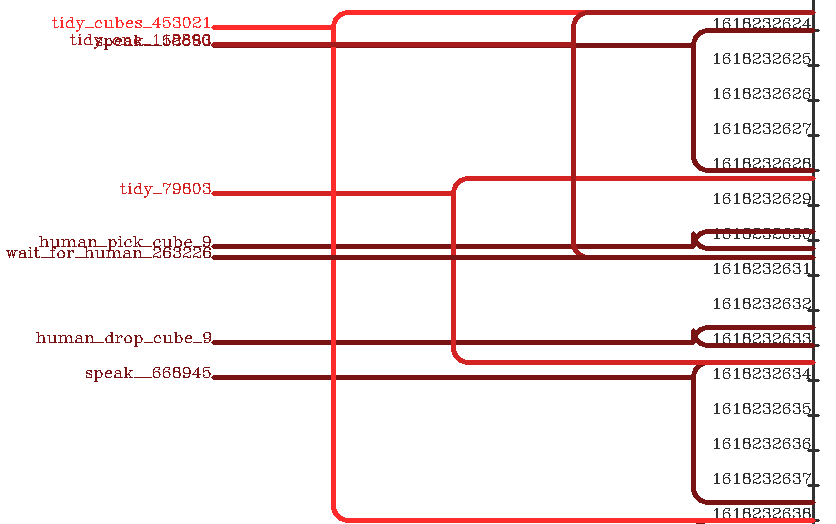
\includegraphics[width=\linewidth]{figures/chapter2/timeline.png}
	\caption{Example of timeline with the Director Task, one cube had to be removed from the shelf by the human. It has been automatically generated by Mementar after having received data from \acrshort{jahrvis}.}
	\label{chap2:fig:timeline}
\end{figure}

Moreover, \acrshort{jahrvis} adds the semantic data associated to a task -- agent and parameters -- to the semantic ontology.

\subsection{Interaction Session Management} \todo{mettre state machine théorique que j'ai faite ? je n'ai pas redeveloppé ce module depuis mummer}
This process handles the interaction sessions. An interaction session is triggered when a human is close enough to start a conversation and seems willing to, \ie when the fact  \fact{isEngagedWith}{human\_i}{robot} is added to the knowledge base and sent to \acrshort{jahrvis}. In this way, the robot tries to respect people that does not want to interact with it. From there, the robot is in the first phase of the interaction session, the \textit{greetings}. The robot says hello to the human and announces the activities it can perform with them, depending on the context they are. The interaction manager triggers the tracking of the human's head by the robot head. This has two purposes: to signal the robot's engagement and to monitor the human's actions. This behavior is quite similar to the one described by Satake \etal~\cite{satake_2015_should}. 

An interaction session stays open as long as the human and the robot perform activities together, \ie as long as the human is engaged in the interaction. This engagement is monitored by the robot in different ways: through the predicate \fact{isEngagedWith}{human\_i}{robot} during dialogue phases outside a task and through what is happening during a task. If at some point the human is not perceived for a while or the human says goodbye, then the manager ends the session. In the latter case, the robot replies with goodbyes. Finally, it returns to its home-base if it has one.

\subsection{Human Actions Monitoring}\label{chap2:subsec:h_moni}
In order to coordinate properly, humans monitor each others when they are in a joint action (see Section~\ref{chap1:subsubsec:monitoring}). The robot needs the same kind of process to be able to assess if the human is doing the action of the plan it expects or not. Existing solutions exist to monitor or recognize human actions but none of them matched all our criteria which are: \todo{faire un état de l'art rapide ?}
\begin{bulletList}
	\item it should be easy and quick to add a new action that the robot can monitor
	\item the process should output the action parameters
	\item the process should give information about the action progress, \ie model the action start and progression when possible and not only the end
	\item it needs to be robust to a potentially unreliable perception
	\item an available open-source code 
\end{bulletList}

Thus, we implemented our own model-based solution with an \acrshort{rja} dedicated to \acrfull{ham}. It relies on the action model presented in Section~\ref{chap2:par:act_rep} which it loads at initiation. We chose to base our action monitoring process on human movements and action effects that the robot can observe. As it needs to monitor them, it extracts the predicate types corresponding to those and subscribes to updates about these facts to Ontologenius as explained in Section~\ref{chap2:subsec:know}. 

Continuously, the \acrshort{ham} \acrshort{rja} monitors facts and human movements that are present in the action model, and sends to the \acrfull{hpm} \acrshort{rja} three types of lists of facts: 
\begin{bulletList}
	\item list of actions that may have started that we coined \emph{possibly started actions}
	\item list of actions that may be progressing that we coined \emph{possibly progressing actions}
	\item list of actions that are estimated as finished that we coined \emph{possibly achieved actions} 
\end{bulletList}

Action states are updated according to received facts. When the state of an action changed to \emph{possibly started}, \emph{possibly progressing} or \emph{possibly achieved}, the affected list is updated and sent to the \acrshort{hpm}. 

The algorithm we developed can be depicted in the form of a Finite State Machine representing the state of one action as shown in Figure~\ref{chap2:fig:action_monitoring} and is implemented in ASL (the code is available in Appendix~\ref{app:jahrvis:h_monitoring}). Each transition is triggered by the addition or the deletion of a fact. Using Jason rules -- they are quite similar to Prolog rules, facts are analyzed to see if they match a movement or an effect of a known action. For example, if we look at the Place action example presented in Section~\ref{chap2:par:act_rep}, it expects the fact \fact{rightHandMovingTowards}{Human}{Support} as a movement. Therefore, receiving \fact{rightHandMovingTowards}{human\_4}{table\_2} will match a Place action movement, however, receiving \fact{rightHandMovingTowards}{human\_4}{milk\_bottle\_2} will not, as the milk\_bottle\_2 does not belong to the Support class (but this fact may be useful to monitor another action). 

The transitions of the state machine are described in Table~\ref{chap2:tab:action_monitoring}. 
 
\begin{figure}[!ht]
	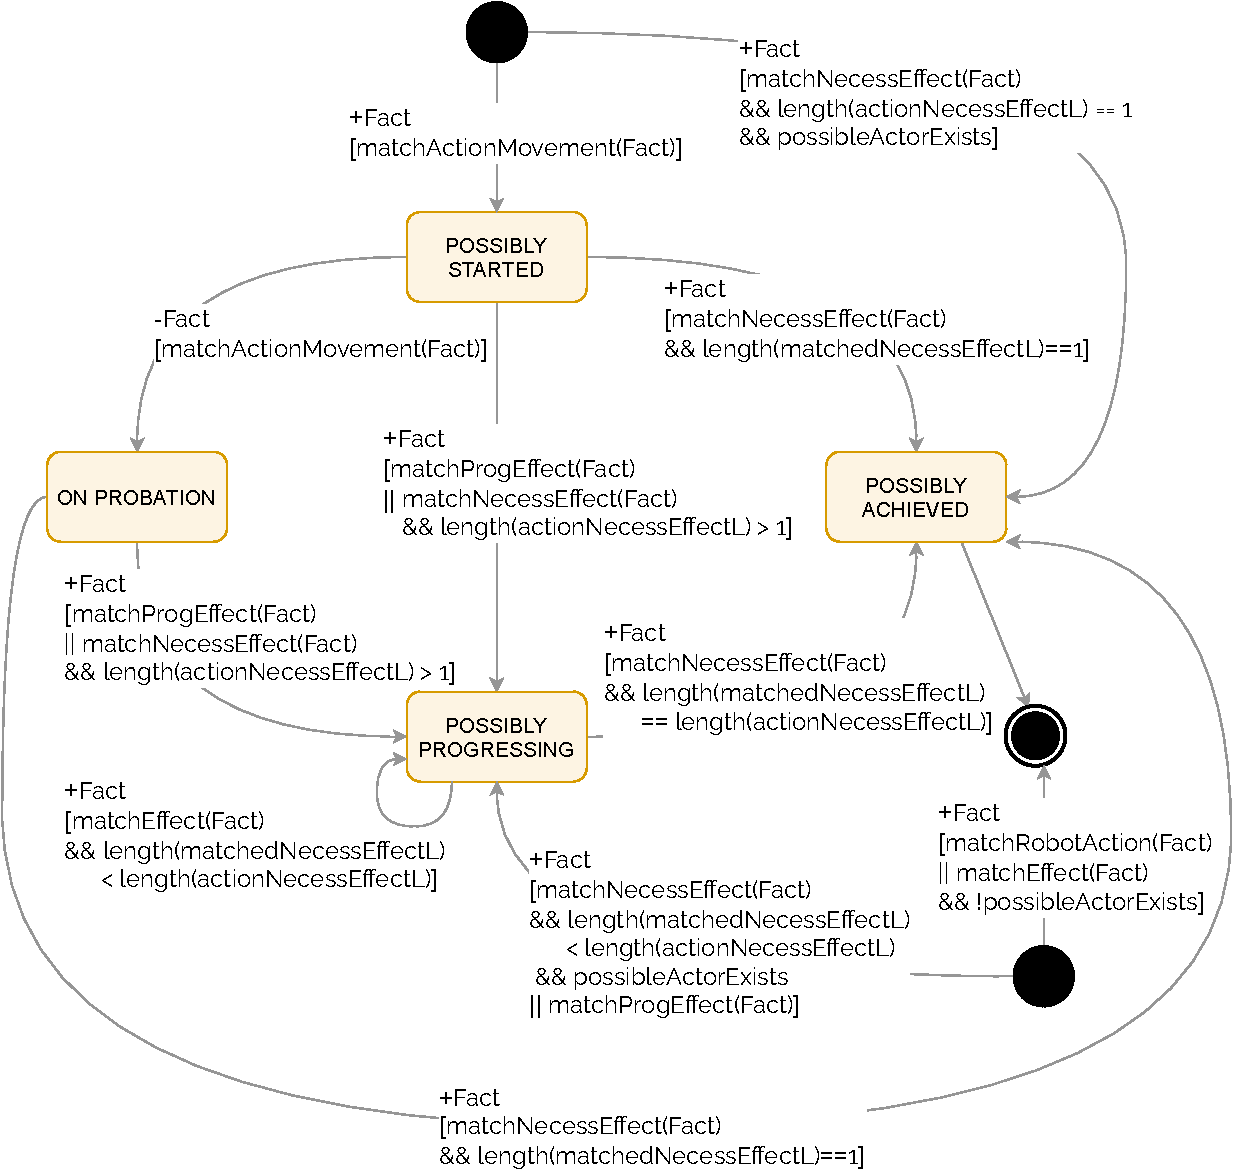
\includegraphics[width=\linewidth]{figures/chapter2/action_sm.pdf}
	\caption{Representation of the \acrfull{ham} \acrshort{rja} in the form of a Finite State Machine representing the state of one action.}
	\label{chap2:fig:action_monitoring}
\end{figure}

\newgeometry{left=1.5in,right=1.3in,top=1.1in,bottom=0.5in,includefoot,includehead,headheight=13.6pt}
\begin{landscape}
	\vspace*{\fill}
	\begin{table}[htb!]
	\caption{Description of the Finite State Machine shown in Figure~\ref{chap2:fig:action_monitoring}.}
	\label{chap2:tab:action_monitoring}
	\begin{tabularx}{\linewidth}{| c | c | c | X |}
		Current State & Input and Condition & Next State & Explanation\\ 
		\hline \hline
	\multirow{4}{*}{Initial State}  & +Fact [matchActionMovement(Fact)] & Possibly Started & When a fact matching a movement for a given action is received, \acrshort{ham} computes that the human may have initiated an action\\  
		\cline{2-4}
		&  \makecell{+Fact [matchNecessEffect(Fact) 
			\\ \&\& length(actionNecessEffectL)	== 1
			\\ \&\& possibleActorExists]} & Possibly Achieved & The robot may have missed the movement or the progression effect of an action because it was not looking or the perception did not detect it. Then when a necessary effect is received and that only one exists for the action, the action is estimated as achieved if it is possible to find an agent who may have performed it.\\  
		\cline{2-4}
		&  \makecell{+Fact [matchNecessEffect(Fact) 
		\\ \&\& length(matchedNecessEffectL)
		\\ < length(actionNecessEffectL)
		\\ \&\& possibleActorExists
		\\ || matchProgEffect(Fact)]} & Possibly Progressing & Similarly to the case above, the robot may have missed the movement or the progression effect of an action. However, if this action has several necessary effects, the action is considered as progressing.\\  
		\cline{2-4}
		& \makecell{+Fact [matchRobotAction(Fact)
		\\ || matchEffect(Fact) \&\& !possibleActorExists]} & Final State & The \acrshort{ham} is aware of the actions executing by the robot so it does not mismatched its action effects with the ones of another agent. If an effect matches, nothing happen. Likewise if an effect is detected but no agent could be found that might have done it.\\  
		\hline 
	\end{tabularx}
\end{table}
\vspace*{\fill}
 \begin{table}[htb!]
 	\caption*{Table~\ref{chap2:tab:action_monitoring}: (continued)}
	\begin{tabularx}{\linewidth}{| c | c | c | X |}
		Current State & Input and Condition & Next State & Explanation\\ 
		\hline \hline
		\multirow{3}{*}{Possibly Started}  
		& \makecell{+Fact [matchProgEffect(Fact)
			\\ || matchNecessEffect(Fact) 
			\\ \&\& length(actionNecessEffectL) > 1]} & Possibly Progressing & When a fact corresponding to a progression effect of the started action is received, or it matches a necessary effect but there are more than one for this action, \acrshort{ham} reinforces its estimation that this action is ongoing by setting it to the progressing state.\\  
		\cline{2-4}
		& \makecell{+Fact [matchNecessEffect(Fact) 
			\\ \&\& length(matchedNecessEffectL) == 1]} & Possibly Achieved 
		& When a fact corresponding to a necessary effect is received and that there is only one for the started action, the action is considered as achieved as the robot is able to observe its effect and that it had observed the human starting it.\\  
		\cline{2-4}
		& -Fact	[matchActionMovement(Fact)] & On Probation & When a movement fact is removed from the belief base without having observed an effect, it might mean that it was a false estimation and that the action is not starting. However, it might also be the robot perception being sporadic and so the action goes in this temporary state waiting for a potential coming effect.\\  
		\hline
	\end{tabularx}
\end{table}
\vspace*{\fill}
  \begin{table}[htb!]
  	\caption*{Table~\ref{chap2:tab:action_monitoring}: (continued)}
	\begin{tabularx}{\linewidth}{| c | c | c | X |}
		Current State & Input and Condition & Next State & Explanation\\ 
		\hline \hline
		\multirow{2}{*}{On Probation} 
		& \makecell{+Fact [matchProgEffect(Fact)
			\\ || matchNecessEffect(Fact)
			\\ \&\& length(actionNecessEffectL) > 1]} & Possibly Progressing & An effect is detected and the action state is resumed.\\
		\cline{2-4}
		& \makecell{+Fact [matchNecessEffect(Fact) 
			\\ \&\& length(matchedNecessEffectL) == 1]} & Possibly Achieved 
		& A necessary effect is detected and as there is only one for this action, it is considered as achieved.\\
		\hline
		\multirow{2}{*}{Possibly Progressing} 
		& \makecell{+Fact [matchNecessEffect(Fact) 
			\\ \&\& length(matchedNecessEffectL)
			\\ == length(actionNecessEffectL)]} & Possibly Achieved 
		& An necessary effect is received and in total, for this action, there was as many necessary effects received as the ones defined for this action.\\
		\cline{2-4}
		& \makecell{+Fact [matchEffect(Fact) 
			\\ \&\& length(matchedNecessEffectL)
			\\ < length(actionNecessEffectL)]} & Possibly Progressing 
		& When an action effect is received and that either it is another progressing or not the last necessary effect expected for the action, the action state remains progressing.\\  
		\hline
		Possibly Achieved & -- & Final State & When an action is estimated as achieved, this is its final state.\\
		\hline
	\end{tabularx}
	
\end{table}
\vspace*{\fill}
\end{landscape}
\restoregeometry

\subsection{Shared Plans Handling}\label{chap2:subsec:plan_handling}
belief divergence before human action (human missed robot action)(sandra) -> com; 
inaction whereas compute human should act -> com;
handle conditional plan (collaborative work with Guilhem Buisan) and handle agent X (two different ways);
extension of Sandra work about agent X with generic object in sparql language (collaborative work with Guillaume Sarthou); 
replan
can work with different HTN-like planer (and others?) after formating with java class. Integration with two planers (tested and working)
\subsubsection{Robot Plan management}
a plan manager for the robot side; 
present algo or state machine
\subsubsection{Human Plan management}
a plan manager for the human side according to human presence/visibilities/reachabilities;
present algo or state machine

\subsubsection{Robot Resource Management}
depending on the robotic platform (pepper arms+head; pr2 needs planer for action manipulation so no arm manager, only head manager)
head manager: when robot execute an action, look the action object; when the robot speaks, look at the human. Programmed through channels.\todo{deplacer presentation dans mummer ici?}

\subsection{Action Execution Management}
action model;
generic algo, just task as input the action model;

\subsection{Communication management}
REG to communicate about actions and objects;
relevant communications;
different communication types (inform executed action, ask to perform action, other informative sentence) (cite Clodic or others?);
human attention

\subsection{Future work}
take preconditions into account to evaluate next action

integrate multiple humans, interaction session handling

improve goal management and interaction session

plan invariants, plans pas entier
 

\section{A robot evaluating its contribution to a human-robot joint action}\label{chap2:sec:qoi}

The work presented in this section has been excerpted from a paper published in the Journal of Social Robotics~\cite{mayima_2021_towards}.

\subsection{Introduction}

Robots dedicated to Human-Robot interactions are not just machines receiving commands and executing them. They should be decisional agents with high-level goals, taking decisions (potentially taking into account social norms), and acting and reacting to not only their actions but those of other agents. Cognitive and interactive robots are becoming more and more capable thanks to the use of human-aware models and algorithms~\cite{kruse2013,thomaz_2016_computational}, with roboticists endowing them with the ability to execute their share of the work while adapting to contingencies, particularly those caused by human's behaviors and decisions~\cite{hoffman_2007_fluency,cakmak_2017,lemaignan_2017_artificial}. The decision-making process is based on a range of knowledge about the environment, the interaction, the context... Nevertheless, curiously and interestingly, very little has been done to allow the robot, while performing its collaborative or assistive activity, to permanently evaluate if things are going well or not, as humans do. We name this ability ``the measure of the Quality of Interaction from the robot point of view''. We believe that enriching the robot knowledge with a good estimation about how the interaction is going, could enhance its decision-making process and thus, its social behaviour.

For example, if the robot detects that the QoI starts to drop, it can take a decision based on this information and act to try to improve the interaction quality (\eg it can choose to change some modalities such as the language in which it communicates with the human, the volume of its speakers, or the parameters of its planners). On the contrary, when the QoI is high, the robot can decide to just continue the interaction as planned. Then, endowed with a QoI Evaluator, a robot becomes more adaptive and performs better. Also, a very poor performance all along a task could allow the robot to assess that the human is not really engaged in the interaction, or even is trying to play the robot. In such situation, the robot might perhaps better disengage. 
Finally, from a methodological point of view, a robot deployed in the wild able to assess interactions, has an asset compared to others as it could reduce the investment in material and human resources to perform user studies. And, a developer might use the logs to improve their design. 

In this paper, we only focus on the Quality of Interaction evaluation process and not on how to use its result for decision making. Therefore,  we present in the sequel the methods and tools we developed, allowing the robot to evaluate in real-time the quality of the human-robot collaborative activity it is involved in. It is based on a set of metrics we have defined, focused on two concepts: the measure of human engagement and the measure of the effectiveness of collaborative tasks performance. However, this is by no means exhaustive, and other metrics and parameters could (and should) be added later. Our work can be seen as a toolbox among which it is possible to pick the desired metrics according to tasks or contexts. We propose a way to aggregate these metrics, producing the QoI. The evaluation of the QoI is performed at three different levels of abstraction: the interaction session level, the task level and the action level. In further work, this ability could provide additional information to the robot and open the possibility for reconsidering its behaviour in case it estimates that the quality of the interaction is degrading (\eg changing its plan or the way it is achieving it, informing the human or requesting a change in their behaviour, or even deciding to disengage).

The section is organized as follows. First, we briefly discuss related work and the main challenges. In section~\ref{chap2:sec:levels} we present the representation of human-robot collaborative activity which we use and its hierarchical  decomposition. Finally, in sections \ref{sec:eval} and \ref{sec:metrics}, we introduce our concept and proposed set of metrics to evaluate the Quality of Interaction.

\subsection{Related work}\label{sec:rel}

Inspired from the evaluation methods used in Human-Computer Interactions and User Experience fields, the field of Human-Robot Interaction (HRI) has elaborated its own methods to evaluate robotic systems when they interact with humans. There are various ways to evaluate a human-robot interaction from the human perspective. Bethel \textit{et al}.~\cite{bethel_2010_review} divided them into five categories: \begin{enumerate*}[label={(\arabic*)}]
	\item self-assessments,\label{list:m_self}
	\item interviews,\label{list:m_inter}
	\item behavioral measures,\label{list:m_beha}
	\item psychophysiology measures, and\label{list:m_physio}
	\item task performance metrics\label{list:m_task}
\end{enumerate*}. They reviewed metrics used for each of the categories. They can be grouped into two types: \ref{list:m_self} and \ref{list:m_inter} are subjective metrics and, \ref{list:m_beha}, \ref{list:m_physio} and \ref{list:m_task} are objective ones. Since our aim is to have a robot able to evaluate interactions by itself, human subjective metrics are not usable. Then we focused on the study of existing objective metrics meant to measure how the interaction goes. Steinfeld \textit{et al}.~\cite{steinfeld_2006_common} proposed a set of metrics to be used in a wide range of tasks whose goal is to assess the system performance by measuring the task effectiveness (\ie how well the task is completed) and the task efficiency (\ie the time required to complete a task). Their work is very thorough and inspiring but does not target the evaluation of the quality of an on-going interaction. 
Hoffman~\cite{hoffman2019} defined a type of quality of interaction, the \textit{fluency}, pointing out that the notion is not well defined and somewhat vague but can still be assessed and recognized when compared to non-fluent scenario. To measure it, they propose a list of objective metrics, only based on duration measures, designed to be quite general: robot idle time, human idle time, concurrent activity (\ie active time of both the robot and the human), functional delay (\ie time difference between the end of one agent’s task and the beginning of the other agent’s task). It is an interesting way to measure the fluency and thus the quality of the human-robot interaction but it only applies to shared workspace tasks and is dedicated to an offline evaluation.

Systems targeting real-time measurements during human-robot interactions, with the purpose to ``close the loop'' and use the information for decision-making, have been developed. Tanevska \textit{et al}.~\cite{tanevska:hal-01615491} proposed a framework allowing the robot to perceive with face detection and evaluate in real-time the affective state (\ie anger, happiness, sadness, surprise, etc) and the engagement state (\ie whether the person is interested or bored in the interaction) of the people it is interacting with. However, the human affective state measure might not be enough to assess an interaction or a task as an affective state is actually a facial expression which can be misinterpreted (\eg a smile can be a sign of happiness or embarrassment) and which might be not visible when one of the agent perform an action and looks somewhere else. Moreover, as the notion of engagement is very task specific, it needs further exploration. Real-time engagement measurement has also been investigated by Anzalone \textit{et al}.~\cite{anzalone_2015_evaluating} using metrics such as gaze, head pose, body pose and response times. Their work is interesting and could be an element among others to assess the interaction quality but, it is dedicated to face-to-face interactions. 

Cameras are not the only sensor used to assess interactions on-the-fly, some use human physiological responses such as skin conductance and temperature, heart or brain signals. Itoh \textit{et al}.~\cite{itoh2006}, Bekele \textit{et al}.~\cite{bekele_2014} or Kulic \textit{et al}.~\cite{kulic2007} use them to detect human affective states such as anxiety or liking in real-time. However, physiological measures often imply a lot of sensors which can be invasive for the human. And, as explained by Kulic and Croft~\cite{kulic_2003_estimating}, physiological signals may be difficult to interpret and there is a large variability in physiological response from person to person. Thus, it can be difficult for a controller to determine which emotional state the subject is in, or whether the response was caused by an action of the system, or by an external stimulus. Moreover, we claim that the human affective state only is not enough to assess the quality of an interaction, a human could be satisfied with an interaction or a task result even though they were stressed during it.

Finally,  Bensch \textit{et al}.~\cite{bensch17} proposed a formal approach to compute interaction quality in real-time. Their work focused on how to combine metrics together which is in the same line as ours. However, they do not provide implementation examples, remaining at an abstract level.

In summary, while a substantial number of studies have been devoted to the evaluation of collaborative interactions for analysis purposes once the interaction is over, there is a lack of methods allowing the robot to evaluate in real-time the quality of the interaction based on multiple metrics and not only anxiety or engagement. We claim that such an ability is very important and should strongly influence the situation assessment as well as the decisional abilities of interactive and collaborative robots. 




\subsection{The Quality of Interaction (QoI)}\label{sec:eval}

We believe the real-time assessment of the Quality of Interaction (QoI) with a human partner (\ie what the robot ``thinks'' about how the interaction is going) is a new knowledge that could enhance the robot decision-making process. We define the Quality of Interaction as a measure that indicates how good is the interaction during human-robot collaborative activities. It is computed in real-time based on a set of metrics, at three different levels: the interaction session level, the tasks level and the actions level. The QoI of a given level is computed from selected metrics but also from the QoIs of the level below as shown in Fig.~\ref{fig:qoi_schema}.

\begin{figure}[!ht]
	\centering
	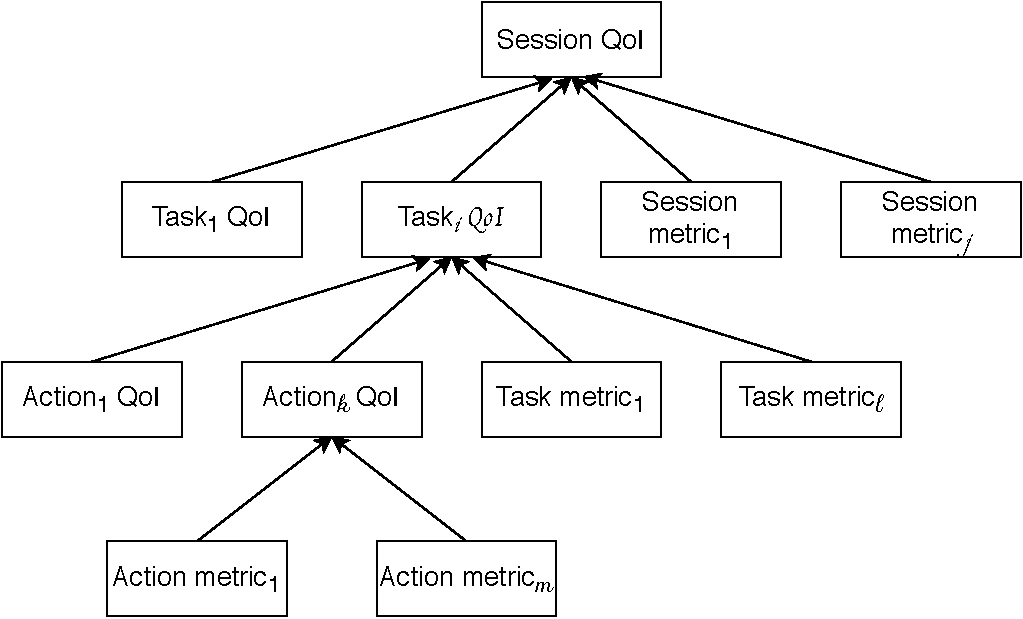
\includegraphics[width=\linewidth]{figures/chapter2/QoI_schema.pdf}
	\caption{Representation of the QoI dependencies, with $i$ the number of performed tasks during the interaction session, $k$ the number of performed actions during the task $i$, $j$ the number of metrics to measure the interaction session QoI, $l$ the number of metrics to measure the task $i$ QoI and $m$ the number of metrics to measure the action $k$ QoI.}
	\label{fig:qoi_schema}
\end{figure}

The QoI of each level is computed as a score between [($1$) for a good quality] and [($-1$) for a poor one]. Metrics used to compute the QoI are divided in three categories: 
\begin{bulletList}
	\item $Mp \in [0,1]$ if it can only have a positive effect on the evaluation;
	\item $Mn \in [-1,0]$ if a metric can only have a negative effect on the evaluation;
	\item $M \in [-1,1]$ if a metric can have a positive or a negative effect.
\end{bulletList}

Defined by the designer according to the needs and context, a metric can belong to one category or another depending on the target application. When needed, metrics values are scaled with the equations presented in Appendix~\ref{annex:functions}.

The evaluation of the Quality of Interaction at the level $l \in \{session_f,task_j,action_k\}$ (with $f,j \text{ and }k$ respectively the identifiers of a given interaction session, task and action),  $QoI_l$, is computed with:

\begin{equation}\label{eq:qoi}
QoI_{l}= \frac{ \sum\limits_{i=0}^x W_i * M_i}{\sum\limits_{i=0}^x W_i} + A * \frac{ \sum\limits_{i=0}^y Wn_i * Mn_i  + \sum\limits_{i=0}^z Wp_i * Mp_i}{\sum\limits_{i=0}^y Wn_i+\sum\limits_{i=0}^z Wp_i} 
\end{equation}


with $W_i, Wp_i,Wn_i$ respectively the corresponding designer-set weights of $M_i, Mp_i, Mn_i$, $A$ the designer-set weight of the right part of the $+$ sign and $x$, $y$, $z$ respectively the number of the metrics $M_i, Mp_i, Mn_i$.

Equation~\ref{eq:qoi} aggregates the values of the metrics chosen to be indicators of the interaction level quality. As all metrics do not have the same importance in the measure of the QoI, each of them is weighted. Values of these weights are empirically defined. There are two parts in the equation, the left part of the $+$ sign and the right part. The left part of the $+$ sign is a weighted mean of the third category of metrics, the $M$ metrics. The right part is a weighted mean of the metrics seen as bonus (\ie $Mp$ metrics) or penalty (\ie $Mn$ metrics). This latter part is weighted with $A$ -- whose value is also empirically\footnote{Values are empirically defined given intuition regarding the importance of a given metrics for a given task and a set of testing experiments} defined -- to be able to adjust its influence on the left part. In such a way, if there are no $Mn$ metrics to compensate for the $Mp$ metrics, it is possible to limit the positive influence of the $Mp$ metrics on the $M$ metrics with $A$. It is the same if there are no $Mp$ metrics, $A$ can compensate the impact of the $Mn$ metrics on the $M$ metrics. Even though $M, Mp, Mn \in [-1,1]$, the final result of $QoI_l$ might be less than $-1$ or greater than $1$ because of the addition of the $M$ with the $Mn$ and $Mp$. If it happens, $QoI_l$ minimal value is set to $-1$ and its maximal value is set to $1$.

\subsection{A set of metrics}\label{sec:metrics}

In this section, we present a few measures to assess the QoI of an interaction session in Sect.~\ref{subsec:m_intersess}. Then, we present metrics for the different levels based on engagement in Sect.~\ref{subsec:m_engag} and effectiveness estimations during human-robot joint activities in Sect.~\ref{subsec:task_eff}. For example, if the human is engaged and if tasks are performed effectively, the QoI will tend to be high and \textit{vice versa}. Both concepts are difficult to measure, so we do not exactly measure them but we compute their trends from the set of metrics presented in this section. This set is not exhaustive and will be extended in future work but it gave promising results as we show with our implementation in Chapter~\ref{chapter:chap3}. All metrics are meant to be used for online evaluations of interactions. They are summarized in Table~\ref{tab:theo_metrics}.

\begin{table*}[t]
	\centering
	\begin{tabular}{|c|p{0.5cm}|p{3cm}|p{3.5cm}|c||c|c|c|}
		\hline
		&  \multicolumn{2}{c|}{Metric names} & Measures & Illustration & Session & Task & Action \\
		\hline\hline
		\multirow{10}{*}{\rotatebox[origin=t]{90}{Effectiveness}} & \multirow{6}{*}
		{\rotatebox{90}{Progress towards goal}} & Distance-to-Goal  & Geometric distance & \parbox[c]{3.5cm}{
\includegraphics[width=3.5cm]{figures/chapter2/dtg.png}} & & x & x \\\cline{3-8}
		& & Time-to-Goal & Time & \parbox[c]{3.5cm}{
\includegraphics[width=3.5cm]{figures/chapter2/ttg.png}} & & x & x\\\cline{3-8}
		&  & Steps-to-Goal & Number of executed actions/substasks & \raisebox{-0.3cm}{\parbox[c][1.5cm]{3cm}{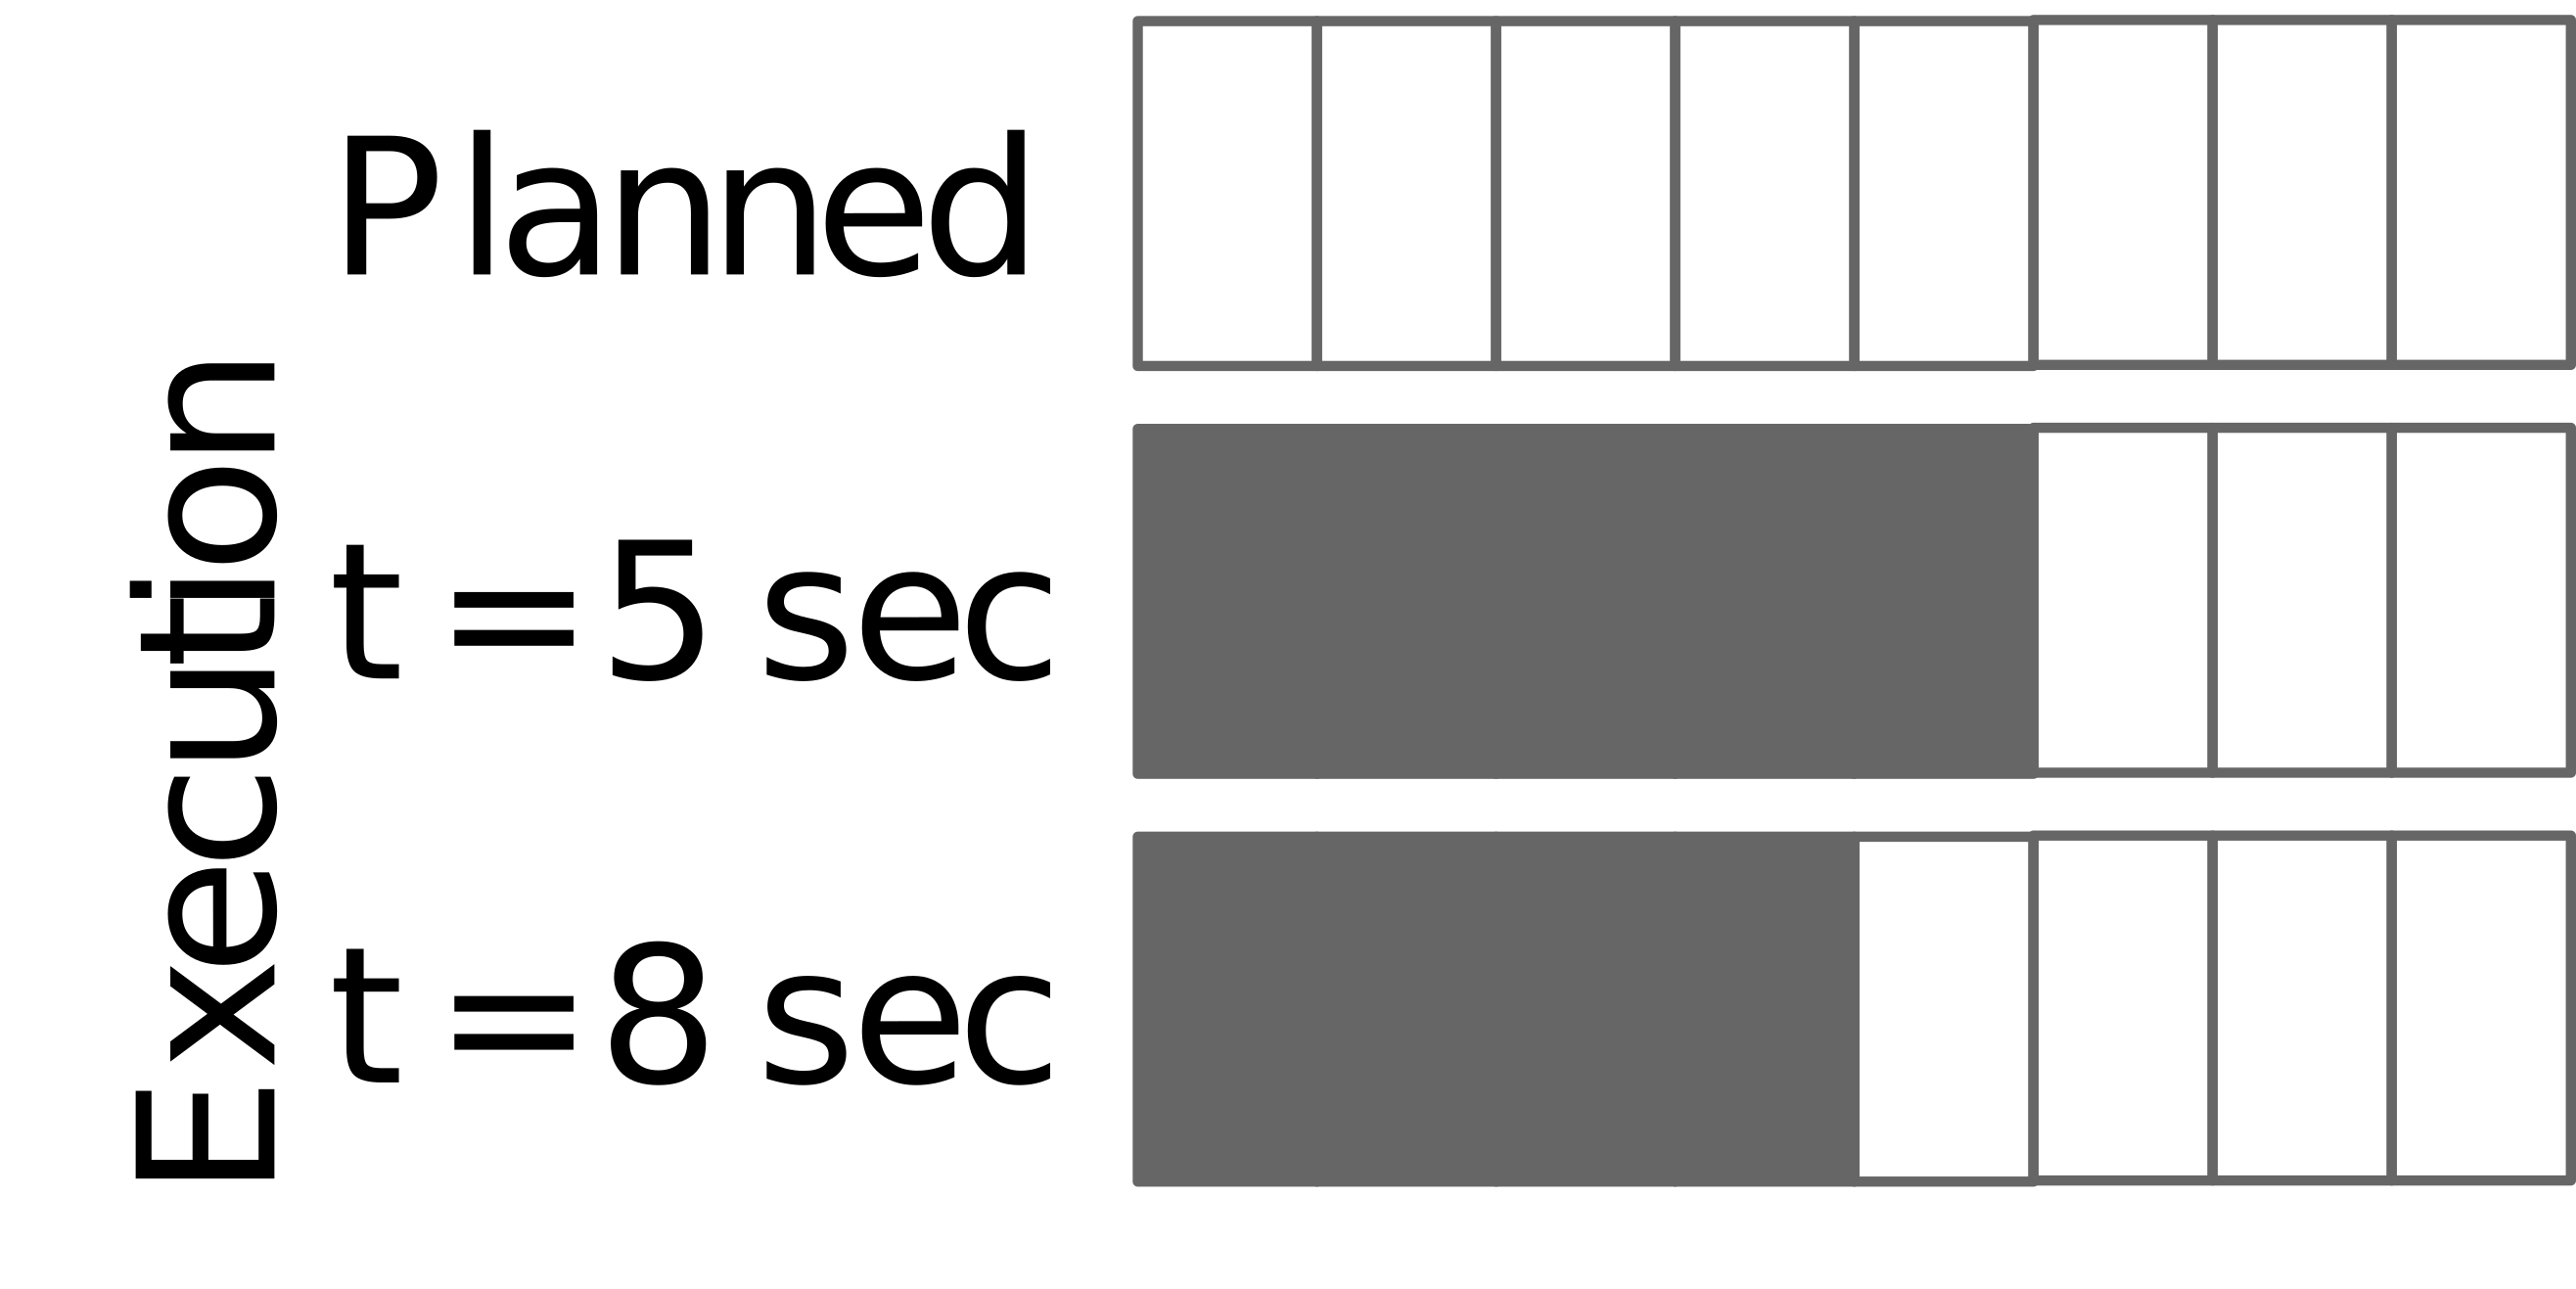
\includegraphics[width=3cm]{figures/chapter2/stg.png}}}&  & x &  \\\cline{2-8}
		&  \multicolumn{2}{p{3.5cm}|}{Deviation from standard duration} & Time & \parbox[c][1.2cm]{3.5cm}{
\includegraphics[width=3.5cm]{figures/chapter2/dd.png}}& & x & x \\\hline
		\multirow{5}{*}{\rotatebox[origin=c]{90}{Engagement}} 
		&  \multicolumn{2}{p{3.5cm}|}{Fulfilling robot expectations about social interaction} & \eg attention ratio, with-me-ness,... & \raisebox{-0.6cm}{
\includegraphics[width=3.5cm]{figures/chapter2/ar.png}}&x & x & x \\\cline{2-8}
		&  \multicolumn{2}{p{3.5cm}|}{Human contribution to the goal} & \eg number of repeated instructions, number of successful human actions,... & \raisebox{-0.8cm}{{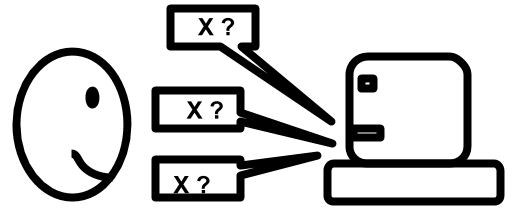
\includegraphics[width=2.4cm]{figures/chapter2/cg.png}}} & & x & x \\\hline
		% &  \multicolumn{2}{c|}{Interaction continuation} & \eg duration, number of tasks/actions, termination manner & x & x & \\\hline
	\end{tabular}
	\caption{The set of metrics presented in Section~\ref{sec:metrics}.}
	\label{tab:theo_metrics}
\end{table*}     


\subsubsection{Measures to assess the QoI at the interaction session level}\label{subsec:m_intersess}
According to the context, the duration of an interaction session can be an indicator of the human engagement. Indeed, a human leaving only a few seconds after the beginning of the interaction is probably less engaged than a human staying with the robot several minutes. Also depending on the context, the number of executed tasks is a measure which can be considered as interesting information with respect to the engagement of the human, as well as the ratio of successful tasks. The more the human executes successful tasks with the robot, the higher the session QoI might be. Finally, it can be valuable to take into account how the session has been terminated in the evaluation of the quality of an interaction session. For instance, the fact that the human leaves abruptly in the middle of a task, during an idle time or a conversation without saying goodbye, or only at an appropriate time saying farewell to the robot is significant in terms of social interaction quality.

\subsubsection{Metrics related to human engagement}\label{subsec:m_engag}
Michael \textit{et al.}~\cite{michael2016} stated that commitments\footnote{In the robotic domain, it is the word ``engagement'' and not ``commitment'' which is often used, unlike in the psychological and philosophical fields.} facilitates ``the planning and coordination of joint actions involving multiple agents. Moreover, commitment also facilitates cooperation by making individuals willing to contribute to joint actions to which they would not be willing to contribute if they, and others, were not committed to doing so''. As it is an important element of the joint action, we want to provide the robot with a way to estimate the engagement of its partner during an interaction. 

Metrics allowing to state if an agent is engaged or not in an interaction are often specific to the type of interaction. For example, Fan \textit{et al.}~\cite{fan2017} implemented their measure of the human engagement as a kind of hysteresis: when the human gaze is on the robot, they are considered as engaged and when the human gaze is somewhere else during more than 3 consecutive seconds, they are considered as not-engaged. 

In the same vein, we think that the measure of the engagement for a collaborative activity can be divided in 2 types of metrics, summed up in Table~\ref{tab:theo_metrics}: the Human contribution to the goal and the Fulfilling robot expectations about social interaction.

We define in this section examples of metrics of each types which can be used to estimate the level of engagement of the human partner. 

\paragraph{Human contribution to the goal}\label{subsubsec:h_contrib}

A good and very promising indicator could be the ability from the robot to evaluate how well the human actions help to the goal progression. We call this indicator \textit{Human contribution to the goal}. To the best of our knowledge, there is no general method to estimate it. 

As a first version of the \textit{Human contribution to the goal}, we chose to measure it through the number of times the robot has to repeat an instruction or a question before the human performs correctly, when it expects the human to answer or to perform the action. As, if it needs to repeat, it means that the human is not correctly contributing to the goal, intentionally or not, as they are not performing their part of the HR action as they should. The more the robot needs to repeat because of the human's bad performance, the less they are contributing to the goal, the more the action QoI should decrease. 

\paragraph{Fulfilling robot expectations about social interaction}\label{subsubsec:r_exp}
During a social interaction, agents are expected to behave in a certain way and so the robot has expectations about the human. Then, the robot can monitor the human behavior to check if they are acting as they are expected to. For example, most of the time, when the robot speaks to the human, it will expect them to look at it and so it can monitor if it is the case or not as implemented by Fan \textit{et al.}~\cite{fan2017}. Quite similarly, Lemaignan \textit{et al.}~\cite{lemaignan2016} developed a way to measure if the human is \textit{with} the robot during their interaction, based on attention assessment, by computing if the human is looking at the desired attentional target or not. This latter metric will be integrated to our framework in future work.

As the works of Lemaignan \textit{et al.} and Fan \textit{et al.}, we estimate the \textit{Fulfilling robot expectations about social interaction} with the human head orientation, in the context of our implementation described in Chapter~\ref{chapter:chap3}. We compute an attention ratio \ie the time during which the human is attentive to the robot (\ie staying close enough and looking at it) when it speaks compared to the total time of the speech:

\begin{equation}\label{eq:attention_r}
Ar = \frac{duration_{isAttentiveTo(robot)=true}}{duration_{robot\_speaks}}
\end{equation}

\paragraph{Metrics related to effectiveness}\label{subsec:task_eff}
One can elaborate metrics to measure how well a task or an action is achieved. As discussed by Olsen and Goodrich~\cite{olsen_2003_metrics}, there are a variety of metrics such as time-based metrics which reward the speed of performance or the response times; error metrics which are based on counting retrials, failures, or mistakes; coverage metrics which measure to what extent a goal is achieved, as well as other possible metrics. We use some of them such as counting retrials, however these metrics alone were not enough for our example task as we are in a HRI context.

One can measure for different kinds of tasks, the ratio of successful\footnote{Obviously, the success is context and task dependent and should be defined according to the needs} executions to the total number of executions (\eg $R=\dfrac{Succ}{Exec}$) or the deviation from the initial plan (distance, cost, trajectory, etc). 

We define four metrics, summed up in Table~\ref{tab:theo_metrics}, allowing to measure the current task and action effectiveness. Three of them are means to measure how the progress towards the goal of a task or an action varies. Indeed, they are good indicators for the interaction quality as, when executing a task or an action, if the agents are not getting closer from the goal or even diverged from it, it means that something goes wrong. There are three different metrics because the one to use depends on the type of task or action. The fourth metric allows to compare the current execution duration to the standard execution duration of the task or action, based on durations measured during previous executions.

\paragraph{Metrics to assess the progress towards the goal}

We defined three different metrics to assess the progress towards the goal. The first one allows to assess the progress towards the goal of geometric-based actions. The second estimates the progress by using the remaining time to reach the goal. Finally, the last one measures the number of remaining steps (actions or substasks) before achieving the goal of a task.

\subparagraph{Distance-to-Goal}\label{para:dtg_gd} 
When an agent is performing a geometric-based action such as a movement, observing if the agent is getting closer to the target position over time provides a useful information about how well the action is going. Therefore, we introduce the \textit{Distance-to-Goal} $\Delta DtG$ metric: 
\begin{equation}\label{eq:dtgg}
\left\{
\begin{array}{ll}
\Delta DtG(t=0) = 0\\
\begin{aligned}
\Delta DtG(t) &= \max(0,\Delta DtG(t-1) - 1)  \\&\text{if } path\_length(t) <  path\_length(t-1) \\

\end{aligned}\\
\Delta DtG(t)= \Delta DtG(t-1) + 1, \text{otherwise.}

\end{array}
\right.
\end{equation}
with $path\_length(t)$ the length of the path leading the goal at time $t$ (\eg which can be given by a reactive motion planner~\cite{khamb2019}). The metric lower bound is 0. If at time $t$ the agent is closer to its final position than at $t-1$, \ie progressing towards their goal, the metric is set to decrease or to remain equal to 0. Now, if the agent has not moved or is even further, the metric increases. The closer the metric value is to 0, the better it is, as it means the distance to the goal has decreased over time. We chose to not directly compute the difference between  $path\_length(t)$ and  $path\_length(t-1)$ as the results would be very different whether it is an action implying a long path or a short path. 

\subparagraph{Time-to-Goal}\label{para:dtg_t}
This measure is intended to estimate the progress of a given task or action towards its goal based on the estimation of the remaining time to reach it. It compares the current estimated time to goal with the initial estimated time to goal taking into account the current task duration. As so, it is possible to measure the variation compared to the initial plan. We define the \textit{Time-to-Goal} $\Delta TtG$ as:
\begin{equation}\label{eq:ttg}
\Delta TtG(t) = \max(0, e(t)  + TtG(t) - TtG(T_0))
\end{equation}
with $e(t) = t - T_0$ the task execution duration (time elapsed since the beginning of the task), $TtG(t)$ the current time to the goal, and $TtG(T_0)$ the initial planned time to goal. In our work, $TtG(t)$ and $TtG(T_0)$ are provided by a reactive motion planner~\cite{khamb2019} because we used the metric for navigation but it could be provided by other kind of planners. 

\begin{figure}[!htb]
	\centering
	% Maximum length
	\subfloat[Plot of $\phi(t)_{X}$ of the subtask $X$ lasting 60 seconds, with $SD_{X}=10 sec$, $V_{X}=0.5$ and $\alpha=1$]{\label{fig:oteX}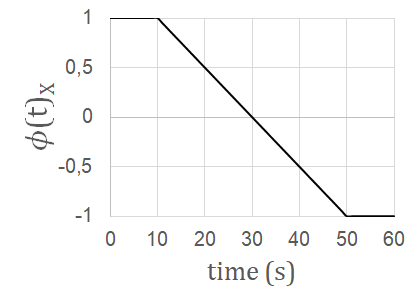
\includegraphics[width=0.49\linewidth]{figures/chapter2/oteX_2.png}}\hfill
	\subfloat[Plot of $\phi(t)_{Y}$ of the subtask $Y$ lasting 15 seconds, with $SD_{Y}=5 sec$, $V_{Y}=1$ and $\alpha=0.5$]{\label{fig:oteY}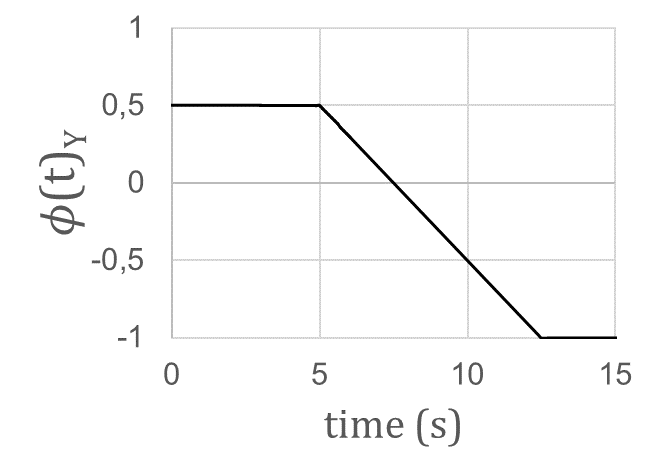
\includegraphics[width=0.49\linewidth]{figures/chapter2/oteY_2.png}}\hfill
	\subfloat[Plot of $\Phi(t)_{Ta}$ for a task composed of a sequence of three subtasks $X, Y, Z$: the duration of $X$ exceeded $SD_X=10 s$ and reached $20 s$, the duration of $Y$ exceeded $SD_Y= 5s$ and reached $10 s$, finally the duration of $Z$ was less than $SD_Z=10s$]{\label{fig:ote2}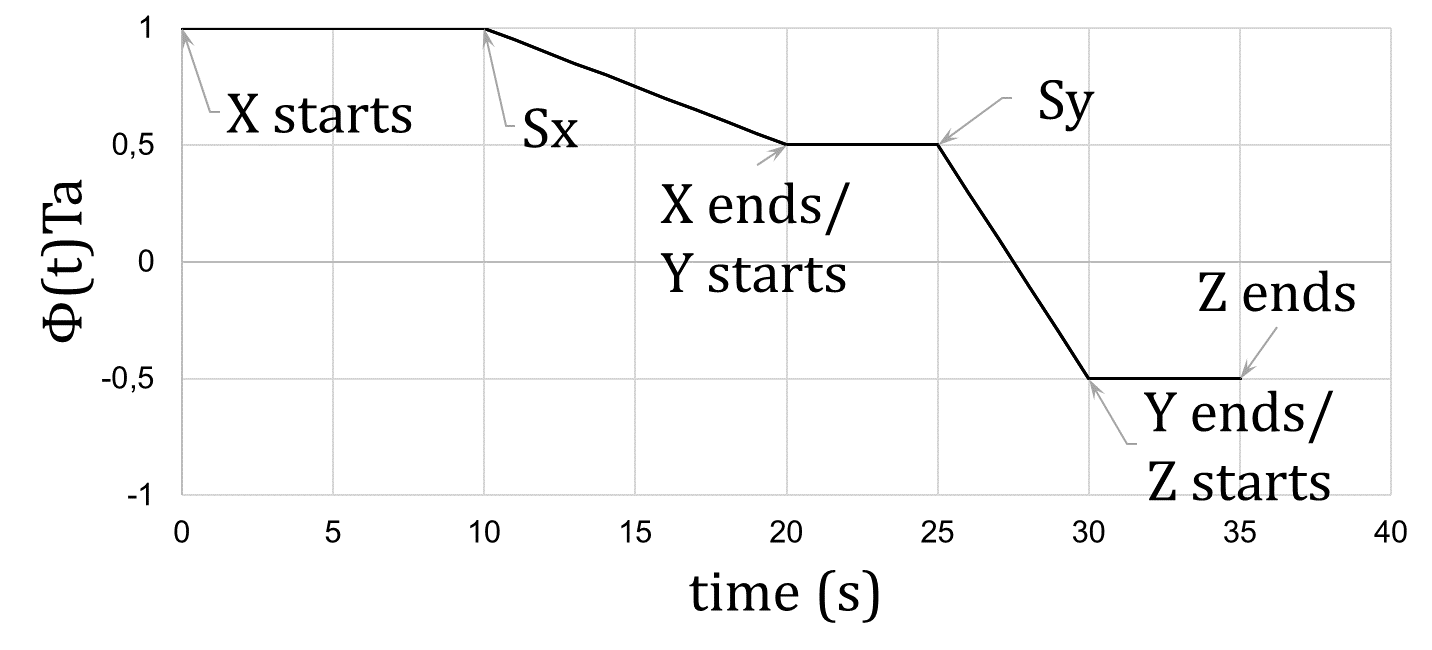
\includegraphics[width=0.7\linewidth]{figures/chapter2/ote.png}}\hfill
	\caption{Examples of plots of the $\phi$ and $\Phi$ functions}
	\label{fig:ote}
\end{figure}

\subparagraph{Steps-to-Goal}
One way to estimate the remaining distance to the goal for a task is to count the number of remaining substasks or actions (depending on the relevant scale) to perform. In addition, one can add a factor which estimates the weight (or effort needed) of each action or subtask. These weights can be determined by the designer, provided by the planner, etc. 
Then, the \textit{Steps-to-Goal} $\mathcal{D}$  of a task can be computed as time $t$:
\begin{equation}\label{eq:edtgs}
\mathcal{D}(t) = \dfrac{\sum\limits_{i=1}^c \mathcal{W}_i}{\sum\limits_{i=1}^n \mathcal{W}_i}
\end{equation}
with $\mathcal{W}_i$ the weight of a subtask/action $i$, $c$ the number of completed subtasks/actions and $n$ the total number of planned subtasks/actions.

\paragraph{Deviation from standard duration}\label{subsubsec:ote}
We introduce here a metric to measure the deviation from standard execution duration, the \textit{Deviation from standard duration} $\phi$ for subtasks/actions and the \textit{Deviation from standard duration} $\Phi$ for a whole task. This measure is intended to represent the degradation of the quality of execution of a HR task when its duration exceeds a certain time. 

To each subtask/action $a_i$, we associate two attributes whose values are defined by the designer: a soft deadline $SD_i$ and a decreasing quality  speed $V_i$. 
If, at time $t$, the execution duration  $e(t) = t - T_0$ of a substask or action $a_i$ which has started at $T_0$ exceeds $SD_i$, the quality will decrease over time at speed $V_i$: 
\begin{equation}\label{eq:ote}
\phi(t)_i=\max\left( V_i*\frac{-\max(e(t)-SD_i,0)}{SD_i}+\alpha,-1\right)
\end{equation}
where $\alpha$ is the value initial value and the upper bound (as at $t=0$, $\max(e(t)-SD_i,0)=0$) of $\phi_i$, when the subtask/action $a_i$ starts.

Then, we define a metric $\Phi$ for a task. It is an aggregation of the $\phi_i$ computed for each performed subtask/action $a_i$ of the task. At any moment, $\Phi$ can be seen as a memory of the previous steps, so the initial value $\alpha$ of $a_i$ is equal to the final value of $\phi_{i-1}$ of the previous subtask/action $a_{i-1}$, $\alpha=\phi(T_{final})_{i-1}$.


We can notice that it is not possible for this metric to increase over time since it memorizes the values of the previous actions. However, the total computed QoI can get higher thanks to the other metrics. Moreover, $\phi$ can be used independently of $\Phi$. In such a case, the initial of value $\alpha$ of $\phi$ can be set to 1. 

Three examples are given in Fig.~\ref{fig:ote}. Fig.~\ref{fig:oteX}~and~\ref{fig:oteY} represent $\phi(t)_{X}$ and $\phi(t)_{Y}$ for two independent subtasks $X$ and $Y$. Fig.~\ref{fig:ote2} is a plot of $\Phi(t)_{Ta}$ for the task $Ta$ composed of the subtasks $X, Y, Z$ with $SD_X=10 s$, $V_X=0.5$, $SD_Y=5 s$, $V_Y=1$, $SD_Z=10 s$ and $V_Z=1$. 

\ifdefined\included
\else
\bibliographystyle{acm}
\bibliography{These}
\end{document}
\fi
